% !TEX program = pdflatex
\documentclass[11pt]{article}

% ---------------------------------------------------------------- fonts and page
\usepackage[T1]{fontenc}
\usepackage[utf8]{inputenc}
\usepackage[scaled=1.0]{XCharter}
\usepackage[scaled=0.95]{sourcesanspro}
\usepackage[scaled=0.98]{inconsolata}
\usepackage{microtype}
\usepackage[letterpaper,top=1in,bottom=1in,left=1in,right=1in,headsep=14pt]{geometry}

\usepackage[table]{xcolor}
\usepackage{booktabs}
\usepackage{tabularx}
\usepackage{array}
\usepackage{longtable}
\usepackage{placeins}
\usepackage{enumitem}
\usepackage{titlesec}
\usepackage{fancyhdr}
\usepackage[font={small,sf},labelfont=bf,labelsep=period,skip=6pt]{caption}
\usepackage[most]{tcolorbox}
\usepackage{graphicx}
\usepackage{amssymb}
\usepackage{multicol}
\usepackage{CJKutf8}   % a few recipe titles contain Chinese
\usepackage[hidelinks]{hyperref}

% ---------------------------------------------------------------- colours
\definecolor{accent}{HTML}{1F5A7A}
\definecolor{ink}{HTML}{1F2933}
\definecolor{muted}{HTML}{5F6B76}
\definecolor{rule}{HTML}{C9D1D9}
\definecolor{tint}{HTML}{F1F5F8}
\definecolor{google}{HTML}{2A78D6}
\definecolor{deepseek}{HTML}{EB6834}
\definecolor{tie}{HTML}{CBD2D9}
\color{ink}

% ---------------------------------------------------------------- spacing
\setlength{\parindent}{0pt}
\setlength{\parskip}{5pt plus 1pt}
\linespread{1.04}
\setlist{itemsep=2pt,topsep=3pt,parsep=0pt,leftmargin=1.5em}
\renewcommand{\arraystretch}{1.32}
\setlength{\tabcolsep}{6pt}
\setlength{\LTleft}{0pt}\setlength{\LTright}{0pt}\setlength{\LTcapwidth}{\linewidth}\setlength{\LTpre}{8pt}\setlength{\LTpost}{6pt}
\newcolumntype{L}{>{\raggedright\arraybackslash}X}
\newcolumntype{P}[1]{>{\raggedright\arraybackslash}p{#1}}
\newcommand{\hd}[1]{\leavevmode\sffamily\bfseries\color{ink}#1}
\newcommand{\headrow}{\rowcolor{tint}}
\newcommand{\id}[1]{\texttt{#1}}

% results tables: a bar of scenarios won (Google | ties | DeepSeek, 1.2 mm per scenario) and winner cells
\newcommand{\winseg}[2]{\textcolor{#1}{\rule[-0.6pt]{\dimexpr 1.2mm*#2\relax}{6pt}}}
\newcommand{\winbar}[3]{\makebox[1.3em][r]{\sffamily\footnotesize #1}\hspace{4pt}%
  \winseg{google}{#1}\hspace{1.2pt}\winseg{tie}{#2}\hspace{1.2pt}\winseg{deepseek}{#3}%
  \hspace{4pt}\makebox[1.3em][l]{\sffamily\footnotesize #3}}
\newcommand{\cg}{\cellcolor{google!24}\leavevmode{\sffamily G}}
\newcommand{\cd}{\cellcolor{deepseek!28}\leavevmode{\sffamily D}}
\newcommand{\ct}{\cellcolor{tie!45}\leavevmode{\sffamily\textcolor{muted}{=}}}
\newcommand{\key}[2]{\textcolor{#1}{\rule[-0.6pt]{7pt}{6pt}}\,#2}
\newcommand{\NScenarios}{20}
\newcommand{\NRuns}{40}
\newcommand{\DomDeepseek}{3}
\newcommand{\DomGoogle}{0}
\newcommand{\DomTradeoff}{17}
\newcommand{\NutrDeepseekWins}{17}
\newcommand{\DecideDeepseekWins}{18}
\newcommand{\DecideGoogle}{2:58}
\newcommand{\DecideDeepseek}{1:30}
\newcommand{\NutrGoogle}{0.40}
\newcommand{\NutrDeepseek}{$-$2.10}
\newcommand{\ShopGoogleWins}{11}
\newcommand{\ShopDeepseekWins}{6}
\newcommand{\PrepGoogleWins}{11}
\newcommand{\PrepDeepseekWins}{6}
\newcommand{\PriceGoogleWins}{10}
\newcommand{\PriceDeepseekWins}{10}
\newcommand{\TasteGoogleWins}{7}
\newcommand{\TasteDeepseekWins}{7}
\newcommand{\TasteTies}{6}
\newcommand{\TasteGoogle}{3.23}
\newcommand{\TasteDeepseek}{3.33}

% table rows are generated by code/results/analyze_baselines.py; the primitive \input keeps booktabs rules happy
% appendix: recipe texts
\newcommand{\zh}[2]{\begin{CJK}{UTF8}{#1}#2\end{CJK}}
\newcommand{\smallfrac}[2]{\textsuperscript{#1}\kern-0.08em/\kern-0.05em\textsubscript{#2}}
\newcommand{\recipe}[3]{\par\addvspace{7pt}\noindent
  {\sffamily\bfseries\footnotesize\color{accent}#1\hspace{0.5em}\color{ink}#2}\par\nopagebreak
  \noindent{\sffamily\scriptsize\color{muted}#3}\par\nopagebreak\vspace{1.5pt}\noindent\ignorespaces}
\makeatletter\newcommand{\rowsfrom}[1]{\@@input #1 }\makeatother

% ---------------------------------------------------------------- headings
\titleformat{\section}{\sffamily\bfseries\Large\color{ink}}{\textcolor{accent}{Part \thesection}}{0.6em}{}
\titlespacing*{\section}{0pt}{16pt plus 3pt}{5pt}
\titleformat{\subsection}{\sffamily\bfseries\large\color{ink}}{\textcolor{accent}{\thesubsection}}{0.6em}{}
\titlespacing*{\subsection}{0pt}{11pt plus 2pt}{2pt}
\newcommand{\lead}[1]{{\sffamily\bfseries\color{accent}#1}\hspace{0.5em}}

% ---------------------------------------------------------------- header and footer
\pagestyle{fancy}
\fancyhf{}
\renewcommand{\headrulewidth}{0pt}
\fancyhead[L]{\sffamily\footnotesize\color{muted}Team J2IS \textperiodcentered{} Meal Prep Advisor}
\fancyhead[R]{\sffamily\footnotesize\color{muted}10-718 \textperiodcentered{} Baselines}
\fancyfoot[C]{\sffamily\footnotesize\color{muted}\thepage}

% ---------------------------------------------------------------- boxes
\tcbset{
  card/.style={enhanced, colback=white, colframe=rule, boxrule=0.6pt, arc=2pt,
               left=9pt, right=9pt, top=7pt, bottom=7pt, before upper={\setlength{\parskip}{5pt}},
               fonttitle=\sffamily\bfseries\small, coltitle=white, colbacktitle=accent,
               toptitle=3pt, bottomtitle=3pt, titlerule=0pt},
  note/.style={enhanced, colback=tint, colframe=tint, boxrule=0pt, arc=2pt,
               left=10pt, right=10pt, top=7pt, bottom=7pt}
}

\begin{document}
\thispagestyle{plain}

% ---------------------------------------------------------------- title
{\sffamily\bfseries\fontsize{22}{26}\selectfont Baselines for the Meal Prep Advisor\par}
\vspace{5pt}
{\sffamily\color{muted}Team J2IS: Jingchu, Jeremy, Ignacy, Souraja \quad\textperiodcentered\quad 10-718\par}
\vspace{2pt}
{\sffamily\small\color{muted}Code and data: \href{https://github.com/gaijingchu/ML-Practice}{\color{accent}github.com/gaijingchu/ML-Practice}\par}
\vspace{7pt}
{\color{accent}\hrule height 1.2pt}
\vspace{2pt}

% Part 1 (revised proposal) goes here.
\setcounter{section}{1}

% ================================================================ Part 2
\section{Evaluation setup}

\subsection{Evaluation set}

We do not train a model for this assignment, so there is no training set and no train/test split.
Every baseline is evaluated on the same fixed set of \textbf{20 scenarios}.
A scenario is a short description of what a user wants to eat, with their preferences and constraints, for example
``Fish meal prep recipes, calories per meal less than 600''.

\textbf{All data in this report were collected by the four members of our group.}
Each member acted as one user: Jeremy (\id{jeremyti}), Souraja (\id{sourajak}), Jingchu (\id{jgai}) and Ignacy (\id{istepka}).
Each of us wrote down our own five scenarios before running anything,
ran both baselines on those scenarios ourselves, and recorded the measurements for our own runs.
Appendix~\ref{app:scenarios} lists the 20 scenarios with the user who wrote each one.

Each scenario is run once with each baseline, which gives 40 runs.
A run ends when the user has decided on \textbf{one} recipe.
All metrics below are measured on that one recipe, because a user acts on a single meal-prep recommendation at a time.

\subsection{Metrics}

We evaluate in a multi-criteria fashion.
Meal prepping has several stages, is spread over time, and involves several decisions,
so collapsing it into one number would lose most of the relevant information.
We therefore report seven metrics and compare methods across all of them:
one method beats another when it is better across the metrics (Pareto dominance).

Each metric has an \emph{online} definition, which is what a user experiences when they follow a meal-prep plan end to end,
and an \emph{offline} version, which is measured or estimated from the recipe alone.
In this assignment every metric is measured offline. Table~\ref{tab:metrics} gives both.

\begin{table}[!htb]
\small
\begin{tabular}{@{}P{2.5cm} P{4.7cm} P{5.2cm} P{1.3cm} P{1.1cm}@{}}
\toprule
\rowcolor{tint} \hd{Metric} & \hd{Definition} & \hd{Offline measurement} & \hd{Unit} & \hd{Better} \\
\midrule
Grocery shopping time &
Time spent buying the ingredients. A more complex basket takes longer in the store,
and having to go to several stores adds much more. &
Estimated, taking into account how likely it is that all ingredients are available at the user's usual grocery store. &
minutes & lower \\
Meal preparation time &
Actual time it takes to prepare all the meals. &
Estimated from the recipe. &
minutes & lower \\
Price &
How much all the meal-prep ingredients cost. &
Expected cost, computed from the prices on the grocery store's website. &
US\$ & lower \\
Tastiness &
Whether the user liked the food they prepared, on a 0--5 scale. &
The user rates the recipe on the same scale, based solely on the recipe. &
0--5 & higher \\
Nutritional value &
How healthy the meal is. &
UK Ofcom Nutrient Profiling Model score of the recipe, per 100\,g. A score of 4 or more is classified ``less healthy''. &
points & lower \\
Diet violation &
If the user specified a diet: whether the meal violates it. &
Same as online: reported by the user. &
0/1 & lower \\
Time to decision &
Time it takes the user to pick a recipe. &
Stopwatch, from starting to formulate the query until the recipe is chosen. &
min:sec & lower \\
\bottomrule
\end{tabular}
\caption{The seven metrics. All are measured on the one recipe the user chose in a run.}
\label{tab:metrics}
\end{table}

\lead{Tastiness scale.}
0: inedible; 1: bad; 2: neutral; 3: okay, but I would not like to continue cooking it; 4: I would cook it again; 5: amazing.

\lead{Nutritional value.}
The Ofcom model gives a food 0--10 points each for energy, saturated fat, total sugars and sodium (``A'' points),
and 0--5 points each for its share of fruit, vegetables and nuts, its fibre and its protein (``C'' points), all per 100\,g.
The score is A minus C, so a lower score is healthier.
If a food has 11 or more A points, its protein points count only when it also scores the full 5 points for fruit, vegetables and nuts.

Section~\ref{sec:eval} describes who measures each metric and how.

% ================================================================ Part 3
\FloatBarrier
\section{Our baselines}

\subsection{Baseline design}

Both baselines follow the same procedure. Only step~3 differs.

\begin{tcolorbox}[note]
\begin{enumerate}[leftmargin=1.4em, itemsep=1.5pt, topsep=0pt, label=\textbf{\sffamily\color{accent}\arabic*.}]
\item Start the timer.
\item Formulate the query for the scenario.
\item Enter the query into the baseline's interface: \textbf{Google Search} or the \textbf{DeepSeek} chat.
\item Read what comes back and decide on a recipe.
\item Stop the timer. This gives the time to decision.
\item Rate the estimated tastiness of the chosen recipe.
\item Measure grocery shopping time, meal preparation time, price and nutritional value for the chosen recipe (Section~\ref{sec:eval}).
\end{enumerate}
\end{tcolorbox}

A user keeps everything else the same across the two baselines:
the same scenario text, the same grocery store, the same location and the same pantry.

\begin{tcbraster}[raster columns=2, raster equal height, raster column skip=10pt, raster before skip=8pt, raster after skip=4pt]
\begin{tcolorbox}[card, title={A \textperiodcentered{} Non-ML baseline: Google Search}]
\small
\textbf{What the user does.}
Enters the query into Google Search, skips the Google AI Overview, opens the results they find promising,
and picks a recipe from one of the pages.

\textbf{Why it is a good baseline.}
This is what people do today when they look for something to meal-prep, and it costs nothing,
so it is the practice our system has to beat.
We skip the AI Overview so that this baseline contains no language model.
\end{tcolorbox}
\begin{tcolorbox}[card, title={B \textperiodcentered{} ML baseline: zero-shot LLM (DeepSeek)}]
\small
\textbf{What the user does.}
Enters the same query as the prompt, with no system prompt and no examples, and picks a recipe from the answer.

\textbf{Why it is a good baseline.}
An off-the-shelf chatbot is the easiest ML alternative to our system that a user could reach for,
so it shows whether the problem needs anything beyond a general-purpose model.

\textbf{Model.} DeepSeek, web chat interface, with web search off.

\textbf{Prompt.} The scenario text, entered verbatim (Appendix~\ref{app:scenarios}).
\end{tcolorbox}
\end{tcbraster}

\FloatBarrier
\subsection{How we evaluate a baseline}
\label{sec:eval}

Table~\ref{tab:eval} lists, for each metric, who measures it and how.
Each group member measures their own runs.
The user measures three metrics directly.
Shopping time, preparation time and price are estimated by an LLM from a fixed prompt template, which is the same for both baselines.
Nutritional value is computed by code.

\begin{table}[!htb]
\small
\begin{tabular}{@{}P{3.0cm} P{2.4cm} P{10.25cm}@{}}
\toprule
\rowcolor{tint} \hd{Metric} & \hd{Measured by} & \hd{How} \\
\midrule
Grocery shopping time & LLM &
\emph{``I already have (ingredient 1, ingredient 2, ...). Here's my meal prep plan \{plan\}.
I usually go grocery shopping at \{grocery-store-name\} (but I can go to other places if necessary), and I live in \{general location\}.
Calculate the total time to for me to shop for the necessary ingredients I need for this recipe.
Assume that I have standard cooking ingredients like salt and pepper.''} \\
Meal preparation time & LLM &
\emph{``This is my receipe for cooking \{recipe\}, please help me to estimate the time for cooking
Assume that I have standard cooking ingredients like salt and pepper (pasted recipe). Unit: minutes.''} \\
Price & LLM, reading the store's website &
\emph{``I already have (ingredient 1, ingredient 2, ...). Here's my meal prep plan \{plan\},
go on \{grocery-store-name\} website, fetch live prices from the store in \{zipcode/address\} and calculate the total price for ingredients that I need to buy.
Assume \{number of portions\} portions. Assume that I have standard cooking ingredients like salt and pepper.''} \\
Tastiness & User & Rated on the 0--5 scale from the recipe alone, right after deciding on it. \\
Nutritional value & Code & Computed after all runs were finished; see the text. \\
Diet violation & User & The user checks the chosen recipe against their diet. \\
Time to decision & User & Stopwatch, started in step 1 and stopped in step 5. \\
\bottomrule
\end{tabular}
\caption{How each metric is measured. Prompts (in italics) are quoted as used; text in braces is filled in by the user.}
\label{tab:eval}
\end{table}

\lead{Nutritional value.}
We compute the Ofcom score with code instead of asking an LLM for it.
For each chosen recipe, the ingredient list is transcribed into quantities and matched to food-composition data from USDA FoodData Central.
The code converts every quantity to grams, sums energy, saturated fat, sugars, sodium, fibre and protein over the recipe,
divides by the total weight to get values per 100\,g, and applies the Ofcom points tables.
The scoring function reproduces the six worked examples in the official technical guidance.
Ingredients that a recipe lists without a quantity, such as ``salt to taste'', cannot be weighed and are not counted.
The ingredient lines were transcribed with Claude Code and are stored next to the original recipe wording in the repository, so they can be audited.
The code, the data and the full list of assumptions are in \texttt{code/nutrition/}.

% ================================================================ Part 4
\FloatBarrier
\section{First-pass results}

We report every metric of Part~2 for both baselines on the same \NScenarios{} scenarios (\NRuns{} runs).
In line with the multi-criteria evaluation, nothing is collapsed into a single score.

\lead{From the sheet to numbers.}
Time to decision was typed as minutes and seconds.
One user recorded shopping time, preparation time and price as ranges, for which we take the midpoint;
for that user's price we take the cost of the whole packages, which is what has to be paid at the store.
A tie on a metric counts for neither baseline.

\subsection{Scorecard}

Table~\ref{tab:scorecard} gives the mean of each metric over the \NScenarios{} scenarios and,
because every scenario was run with both baselines, the number of scenarios in which each baseline is the better one.

\begin{table}[!htb]
\centering\small\setlength{\tabcolsep}{5pt}
\begin{tabular}{@{}l l l r r r c@{}}
\toprule
\rowcolor{tint} & & & \multicolumn{2}{c}{\hd{Mean}} & & \hd{Scenarios won, of 20} \\
\rowcolor{tint} \hd{Metric} & \hd{Unit} & \hd{Better} & \hd{Google} & \hd{DeepSeek} & \hd{Difference} &
  {\sffamily\scriptsize \key{google}{Google}\ \key{tie}{tie}\ \key{deepseek}{DeepSeek}} \\
\midrule
\rowsfrom{generated/scorecard_rows}
\bottomrule
\end{tabular}
\caption{Scorecard. The better mean is in bold. Difference is DeepSeek minus Google.
The bar counts the scenarios in which Google Search (left) or DeepSeek (right) is strictly better; grey is ties.}
\label{tab:scorecard}
\end{table}

\begin{itemize}
\item \textbf{DeepSeek is clearly better on two metrics.} Users decide faster (\DecideDeepseek{} against \DecideGoogle{} minutes, better in \DecideDeepseekWins{} of 20 scenarios)
      and the chosen recipes score healthier (\NutrDeepseek{} against \NutrGoogle{}, better in \NutrDeepseekWins{} of 20).
\item \textbf{Google Search is more often better on shopping and preparation time} (\ShopGoogleWins{} scenarios against \ShopDeepseekWins{} for each),
      although the means differ by less than two minutes.
\item \textbf{Price and tastiness are a draw.} Each baseline is cheaper in \PriceGoogleWins{} scenarios,
      and each is rated tastier in \TasteGoogleWins{}, with \TasteTies{} ties.
\item \textbf{Diet violations are rare.} There is one in the \NRuns{} runs, with Google Search.
\end{itemize}

\subsection{Pareto comparison}

For a given scenario, one baseline \emph{dominates} the other if it is at least as good on all seven metrics and strictly better on at least one.
Table~\ref{tab:pareto} applies this to every scenario.
\textbf{DeepSeek dominates in \DomDeepseek{} scenarios, Google Search in \DomGoogle{}, and in the other \DomTradeoff{} each baseline wins on some metrics.}
So neither baseline Pareto-dominates the other on our evaluation set: the two sit at different points of the trade-off.

\begin{table}[!htb]
\centering\footnotesize
\setlength{\tabcolsep}{2.5pt}\renewcommand{\arraystretch}{1.12}
\begin{tabular}{@{}P{1.4cm} P{4.45cm} *{7}{>{\centering\arraybackslash}p{0.87cm}} >{\centering\arraybackslash}p{0.42cm} >{\centering\arraybackslash}p{0.42cm} P{1.6cm}@{}}
\toprule
\rowcolor{tint} & & \multicolumn{7}{c}{\hd{Better baseline on each metric}} & \multicolumn{2}{c}{\hd{Wins}} & \\
\rowcolor{tint} \hd{User} & \hd{Scenario} & \hd{Shop} & \hd{Prep} & \hd{Price} & \hd{Taste} & \hd{Nutr.} & \hd{Diet} & \hd{Decide} & \hd{G} & \hd{D} & \hd{Dominates} \\
\midrule
\rowsfrom{generated/scenario_rows}
\bottomrule
\end{tabular}
\caption{Pareto comparison for each scenario. G: Google Search is better; D: DeepSeek is better; =: tie.
Columns follow Table~\ref{tab:scorecard}: grocery shopping time, meal preparation time, price, tastiness, nutritional value, diet violation, time to decision.
All of \id{jeremyti}'s scenarios also ask for under 600 kcal per meal.}
\label{tab:pareto}
\end{table}

Figure~\ref{fig:pareto} shows the trade-offs in the original units.
Each panel plots tastiness against one of the costs for all \NRuns{} runs and marks, for each baseline, the runs that no other run of that baseline beats on both axes.

\begin{figure}[!htb]
\centering
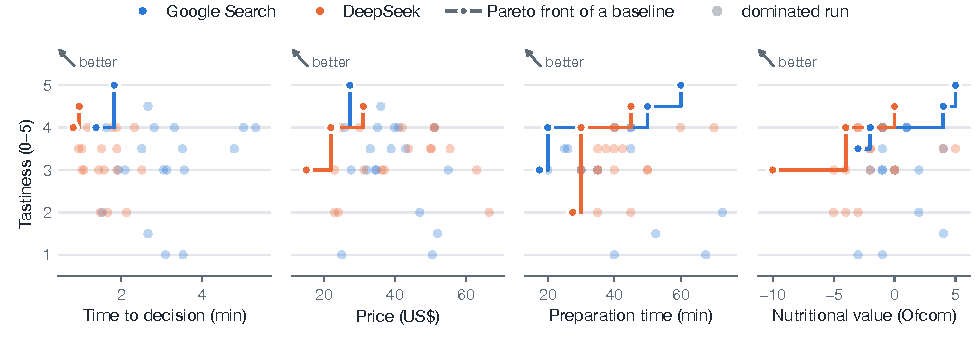
\includegraphics[width=\linewidth]{figures/pareto_tradeoffs.pdf}
\caption{Tastiness against four costs, one dot per run. Lower cost and higher tastiness are better, so the ideal corner is the top left of every panel.
The line joins the non-dominated runs of each baseline in that panel.}
\label{fig:pareto}
\end{figure}

\FloatBarrier
\lead{Caveats.}
These are first-pass, offline measurements.
The users ran the baselines themselves, so they knew which baseline produced each recipe when they rated it.
Shopping time, preparation time and price are LLM estimates.
Part of the nutritional-value gap comes from how the recipes are written:
DeepSeek recipes more often give a quantity for a rice or grain side, which lowers every nutrient per 100\,g,
and salt ``to taste'' cannot be counted for either baseline.
With four users and \NScenarios{} scenarios, small differences in the means should not be read as real.

% ================================================================ Part 5
\section{What this tells us}

\lead{How hard will the baselines be to beat?}
We do not think they will be hard to beat.
The zero-shot LLM has no clear advantage over Google Search:
it dominates Google Search in only \DomDeepseek{} of the \NScenarios{} scenarios, the two are tied on price and tastiness,
and Google Search is more often the better one on shopping and preparation time.
An off-the-shelf model that is asked once is therefore not much better than a web search.
We read this as a sign that the model leaves most of its knowledge unused.
It knows far more about cooking, nutrition and shopping than a single zero-shot answer brings out,
and it is given none of the information that decides price, shopping time and taste for a particular user,
such as live store prices, what the user already has at home, and what they liked before.
A well-built agent and harness around the same base model can bring that knowledge and that information to bear,
so we see room for a large improvement over the base model.

\lead{How much better does our model need to be?}
We would deploy a system that is roughly Pareto-better than \emph{both} baselines:
at least as good as Google Search and as the zero-shot LLM on all seven metrics, and clearly better on at least one.
We say ``roughly'' because, with \NScenarios{} scenarios and several estimated metrics,
we cannot expect it to dominate in every single scenario.
We will judge it on the same scenarios, with the same scorecard and the same per-scenario Pareto comparison as in Part~4.

% ================================================================ Appendix
\clearpage
\appendix
\titleformat{\section}{\sffamily\bfseries\Large\color{ink}}{\textcolor{accent}{Appendix \thesection}}{0.6em}{}
\section{The 20 scenarios}
\label{app:scenarios}

Each group member wrote their own five scenarios and ran them with both baselines.

{\footnotesize\renewcommand{\arraystretch}{1.2}
\begin{longtable}{P{1.6cm} P{1.5cm} P{12.1cm}}
\toprule
\rowcolor{tint} \hd{User ID} & \hd{Anon.\ ID} & \hd{Scenario} \\
\midrule
\endhead
\bottomrule
\endlastfoot
\id{jeremyti} & koala & Asian food meal prep with calories per meal less than 600 \\
      & & Italian food meal prep with calories per meal less than 600 \\
      & & Meal prep recipes that use green onions and ginger, calories per meal less than 600. \\
      & & Fish meal prep recipes, calories per meal less than 600 \\
      & & Meal prep recipe that is tasty and filling, calories per meal less than 600 \\
\midrule
\id{sourajak} & lion & high protein, high fibre, low fat American meal prep recipes without beef \\
      & & Easy and healthy meal prep recipes good for body building with vegetables, chicken, and rice \\
      & & Bengali easy healthy meal prep recipe with vegetables, chicken, and fishes feasible to cook in Pittsburgh \\
      & & Less oily easy healthy and tasty North Indian meal prep recipe with high protein feasible to cook in Pittsburgh \\
      & & Quick and easy high protein South Indian meal prep recipe feasible to cook in Pittsburgh \\
\midrule
\id{jgai} & kangaroo & Chinese food, northern China food, for single person recipe \\
      & & Chinese food, southeast China food, for single person recipe \\
      & & healthy Chinese food, more vegetables, for losing weight recipe \\
      & & U.S Style Chinese food, tasty, for single person recipe \\
      & & Taiwan dishes, single person recipe \\
\midrule
\id{istepka} & hamster & High protein, mexican food. $\dagger$ TVP is fine as meat substitute. \\
      & & Korean vegetarian meal prep with kimchi. $\dagger$ TVP is fine as meat substitute. \\
      & & Tofu \& soy sauce based meal prep. $\dagger$ \\
      & & Broccoli based vegetarian recipes for meal prep. $\dagger$ TVP is fine as meat substitute. \\
      & & Meal prep with gnocchi. $\dagger$ TVP is fine as meat substitute. \\
\end{longtable}
}
\vspace{-6pt}
{\footnotesize $\dagger$ stands for three sentences that appear in each of this user's scenarios:
``I want to meal prep 5 lunches for this week. I don't want to spend too much time in the kitchen.
I do not want to buy any frozen or highly processed food.''\par}
\addtocounter{table}{-1}

\clearpage
\section{Complete results}
\label{app:runs}

Table~\ref{tab:runs} lists all \NRuns{} runs with the values used in Part~4.
Each scenario has two lines, one per baseline. Run IDs (R1--R40) are the ones used in Appendix~\ref{app:recipes}.

\begin{minipage}{\linewidth}
\captionsetup{hypcap=false}\captionof{table}{All runs. Shop: grocery shopping time (min). Prep: meal preparation time (min). Price in US\$. Taste: tastiness (0--5).
Nutr.: nutritional value (Ofcom score). Diet: diet violation (0/1). Decide: time to decision (min:sec).}\label{tab:runs}
\end{minipage}
\vspace{-4pt}
{\footnotesize\setlength{\tabcolsep}{2.6pt}\renewcommand{\arraystretch}{1.1}
\newcolumntype{N}[1]{>{\raggedleft\arraybackslash}p{#1}}
\begin{longtable}{@{}P{0.6cm} P{2.75cm} P{1.72cm} P{3.8cm} N{0.7cm} N{0.7cm} N{0.82cm} N{0.74cm} N{0.74cm} N{0.56cm} N{1.0cm}@{}}
\toprule
\hd{Run} & \hd{Scenario} & \hd{Baseline} & \hd{Recipe chosen} & \hd{Shop} & \hd{Prep} & \hd{Price} & \hd{Taste} & \hd{Nutr.} & \hd{Diet} & \hd{Decide} \\
\midrule
\endhead
\bottomrule
\endlastfoot
\rowsfrom{generated/runs_rows}
\end{longtable}
}
\addtocounter{table}{-1}

\section{The recipes}
\label{app:recipes}

This appendix reproduces the recipe each run ended with, exactly as it was pasted into our sheet
from the web page (Google Search) or from the chat answer (DeepSeek).
Web recipes therefore include page furniture such as photo credits.

\begin{multicols}{2}
\scriptsize\setlength{\parskip}{0pt}\raggedright
\recipe{R1}{Beef and Broccoli}{jeremyti \textperiodcentered{} Asian \textperiodcentered{} Google Search}
Beef and Broccoli Prep Time 14 mins Cook Time 12 mins Resting Time 10 mins Total Time 26 mins Beef and broccoli is a Chinese takeout staple that's easy to make at home. It's fresh, hearty, jam-packed with flavor, and takes less than 30 minutes to make. Course: Main Course Cuisine: Asian, Chinese Keyword: beef and broccoli recipe, beef and broccoli stir fry, chinese beef and broccoli, chinese broccoli Servings: servings Calories: 191 kcal Author: Kelly Ingredients 3/4 pound flank steak , or sirloin, trimmed of fat, very thinly sliced against the grain 1 Tablespoon cooking oil water for blanching broccoli (omit if not blanching) 2 cloves garlic finely minced 1/4 teaspoon grated fresh ginger 3-1/2 cups broccoli florets about 1 head For the Beef Marinade: 1 teaspoon cornstarch , you can use arrowroot or tapioca starch for a corn-free, low carb, Whole30, paleo-version. Omit for keto. 1 teaspoon low sodium soy sauce , can substitute with gluten free tamari or coconut aminos for a Whole30 / paleo-friendly version 1/4 teaspoon dark soy sauce optional for color \& extra flavor (leave out for gluten free, Whole30, keto or paleo version) 1/2 teaspoon toasted sesame oil 1/8 teaspoon black pepper For the Sauce: 1-1/2 Tablespoons oyster sauce , you can also sub with vegetarian flavored oyster sauce use this brand for a Vegan, Keto, Whole30 and Paleo Oyster Sauce. 1-1/2 Teaspoons low sodium soy sauce , you can substitute with gluten free tamari or coconut aminos for a Whole30 / paleo-friendly version. 1/4 teaspoon dark soy sauce , optional for color \& extra flavor (leave out for gluten free, Whole30, keto or paleo version). 2 teaspoons granulated sugar , you can also sub with coconut sugar for paleo or granulated sugar-free sweetener (such as monk fruit sweetener or Swerve for keto). Leave out or swap with homemade date paste (adjusting the amount to taste)or orange juice (adjusting the amount to taste) for Whole30. 1 teaspoon toasted sesame oil 1/2 teaspoon Mirin , can also sub with Chinese cooking wine or dry sherry (omit for paleo and Whole30 version) 2 teaspoons cornstarch , you can use arrowroot or tapioca starch for a corn-free, low carb, Whole30, paleo-version. Use 1/4 teaspoon xanthan gum for keto. salt and black pepper , to taste 1/3 cup cold water or sodium free chicken broth – the chicken broth will add extra flavor, use more as needed to thin out the sauce if needd. Serving Suggestions: cooked rice of choice, cauliflower rice, quinoa, or noodles of choice Instructions Marinate the beef: In a medium bowl, mix together all of the ingredients for the marinade. Add the beef slices and stir until coated. Set aside for at least 10 minutes. Meanwhile blanch the broccoli: (skip if not blanching) In a large non-stick saute pan or wok on high heat, bring the water to a boil. Add the broccoli florets and cook for about 30 seconds. Drain and immediately rinse with cold water to stop the cooking process. Set aside. Make the sauce: Combine all the sauce ingredients together in a small bowl. Set aside. Heat cooking oil over high heat, for about 2 minutes – using the same non-stick pan or wok you used for your broccoli. The pan needs to be hot enough that you start seeing a little bit of smoke rising. Quickly add the beef to the smoking pan and spread the pieces out to a single layer allowing them to sear and brown. Add the garlic + ginger and continue cooking until the meat is no longer pink (about 1-2 minutes making sure not to overcook). Pour in the sauce, stirring constantly, until the sauce boils and thickens – about 30 seconds. Add more water if needed to thin out the sauce. Quickly stir in the broccoli and toss everything together to coat well. Salt and pepper to taste. Sprinkle with sesame seeds and chopped green onions if desired. Serve hot over rice or noodles. For meal prep: Divide evenly into lunch containers with your favorite carb – rice, quinoa or noodles. Recipe Notes Refrigeration: If you find yourself with leftovers, You can keep this dish in a separate airtight container in the fridge for up to 4 days. Meal prep: This dish is also excellent for meal prepping. Divide it into containers along with your choice of rice, quinoa, or noodles. Freezer: You can also store this recipe in an airtight container in the freezer for up to 3 months. Thaw in the fridge before reheating. Reheating: You can use a microwave or heat the stir-fry in a pan or wok over medium heat. Adding a splash of water or broth can help prevent the dish from drying out during reheating.
\par

\recipe{R2}{Japanese Chicken Soba Bowl}{jeremyti \textperiodcentered{} Asian \textperiodcentered{} DeepSeek}
Japanese Chicken Soba Bowl \~{}500 calories | 38g protein | 1 serving A light, broth-based noodle bowl that eats like a big meal but stays well under 600 calories. Ingredients For the bowl: 5 oz chicken breast (or trimmed thigh) 2 oz dry soba noodles 1 cup fresh spinach 1/2 cup shredded carrot 2–3 scallions, sliced Optional: 1/4 cup shelled edamame, 1 soft-boiled egg (adds \~{}70 cal each) For the broth: 2 cups low-sodium chicken broth or dashi 1 tbsp low-sodium soy sauce (or tamari for gluten-free) 1 tsp mirin 1 tsp rice vinegar 1 clove garlic, minced 1 tsp fresh ginger, grated Optional: pinch of chili flakes or a dash of chili oil Instructions Cook the chicken. Season with salt and pepper. Poach in the broth for 12–15 minutes until cooked through (165°F), then shred or slice. Alternatively, pan-sear in a lightly sprayed pan and slice. Make the broth. In a small pot, combine broth, soy sauce, mirin, rice vinegar, garlic, and ginger. Simmer 5–8 minutes. Taste and adjust soy sauce. Cook the soba. Boil per package directions (usually 4–5 minutes). Rinse under cold water—this removes excess starch and keeps the noodles from getting mushy. Drain well. Wilt the spinach. Add spinach and shredded carrot to the hot broth for the last 1–2 minutes, just until spinach wilts. Assemble. Put soba in a bowl, pour broth and vegetables over, top with chicken and scallions. Add chili flakes or a few drops of chili oil if you want heat. Meal Prep Version Store separately: broth, noodles, chicken, and toppings in different containers. Soba absorbs broth and gets soggy if stored together. Reheat: warm broth and chicken together, then add noodles and fresh scallions. Keeps: 3–4 days in the fridge. Calorie Breakdown (approx.) Component Calories Chicken breast, 5 oz 230 Soba, 2 oz dry 190 Broth + seasonings 30 Spinach + carrot 25 Scallions 10 Total \~{}485 That leaves you \~{}100 calories of headroom—enough for a soft-boiled egg or extra edamame without breaking 600.
\par

\recipe{R3}{Frittata Florentine}{jeremyti \textperiodcentered{} Italian \textperiodcentered{} Google Search}
Frittata Florentine Total Time Prep/Total Time: 30 Min. Yield 4 Servings Test Kitchen Approved My family is all about brunchy meals like this gorgeous Italian omelet. Lucky for us, it’s loaded with ingredients we tend to have at the ready. —Jenny Flake, Newport Beach, California Ingredients 6 large egg whites 3 large eggs 1/2 teaspoon dried oregano 1/4 teaspoon garlic powder 1/4 teaspoon salt 1/4 teaspoon pepper 1 tablespoon olive oil 1 small onion, finely chopped 1/4 cup finely chopped sweet red pepper 2 turkey bacon strips, chopped 1 cup fresh baby spinach 3 tablespoons thinly sliced fresh basil leaves 1/2 cup shredded part-skim mozzarella cheese Directions Preheat broiler. In a small bowl, whisk the first 6 ingredients. In an 8-in. ovenproof skillet, heat oil over medium-high heat. Add onion, red pepper and bacon; cook and stir 4-5 minutes or until onion is tender and bacon is cooked. Reduce heat to medium-low; top with spinach. Pour in egg mixture. As eggs set, push cooked portions toward the center, letting uncooked eggs flow underneath; cook until eggs are nearly thickened. Remove from heat; sprinkle with basil, then cheese. Broil 3-4 in. from heat 2-3 minutes or until eggs are completely set. Let stand 5 minutes. Cut into wedges. Nutrition Facts 1 piece: 176 calories, 11g fat (4g saturated fat), 174mg cholesterol, 451mg sodium, 4g carbohydrate (2g sugars, 1g fiber), 15g protein. Diabetic Exchanges: 2 medium-fat meat, 1/2 fat.
\par

\recipe{R4}{Turkey Bolognese with Whole-Wheat Pasta}{jeremyti \textperiodcentered{} Italian \textperiodcentered{} DeepSeek}
Turkey Bolognese with Whole-Wheat Pasta Serves: 5 | Calories: \~{}520 per serving | Protein: \~{}35g Ingredients For the sauce: 1 lb (450g) 93\% lean ground turkey 1 jar (24 oz) no-sugar-added marinara sauce 1 can (14 oz) crushed tomatoes 1 medium onion, diced 2 carrots, diced 2 celery stalks, diced 3 garlic cloves, minced 2 tbsp olive oil 1 tsp dried oregano 1 tsp dried basil 1/2 tsp red pepper flakes (optional) Salt and black pepper to taste For the pasta: 10 oz dry whole-wheat spaghetti Salt for pasta water Instructions 1. Sauté the vegetables (5–6 min) Heat olive oil in a large pot or Dutch oven over medium heat. Add onion, carrot, and celery. Cook until softened, stirring occasionally. 2. Add garlic (1 min) Stir in minced garlic and cook until fragrant. Don't let it brown. 3. Brown the turkey (6–8 min) Add ground turkey, breaking it apart with a spoon. Cook until no longer pink. Season with salt and pepper. 4. Build the sauce (20 min) Add crushed tomatoes, marinara, oregano, basil, and red pepper flakes. Stir to combine. Bring to a simmer, then reduce heat to low and simmer uncovered for 20 minutes, stirring occasionally. 5. Cook the pasta While sauce simmers, bring a large pot of salted water to a boil. Cook spaghetti al dente per package directions (usually 8–10 min). Reserve 1/2 cup pasta water before draining. 6. Combine Toss drained pasta with about 1 cup of the sauce and a splash of pasta water to prevent sticking and coat evenly. 7. Portion and store Divide into 5 containers: \~{}1 cup pasta + \~{}1 cup sauce each. Let cool slightly before sealing. Nutrition Per Serving (approximate) Nutrient Amount Calories \~{}520 Protein \~{}35g Carbs \~{}62g Fat \~{}14g Fiber \~{}10g Sodium \~{}600mg Meal-Prep Tips Storage: Fridge up to 4 days in airtight containers. Freezing: Freezes great — up to 3 months. Freeze sauce and pasta together or separately. Reheating: Microwave 2–3 min, stirring halfway. Add a splash of water if it looks dry. Boost protein: Swap in 99\% lean turkey and add 1/2 cup low-fat ricotta per serving (+\~{}60 cal, +5g protein). Lower carb: Use 6 oz pasta instead of 10 oz, and serve over zucchini noodles for half the portions. More veggies: Add 1 diced bell pepper or 8 oz sliced mushrooms with the other vegetables.
\par

\recipe{R5}{Korean Beef Bowl}{jeremyti \textperiodcentered{} Green onion and ginger \textperiodcentered{} Google Search}
Korean Beef Bowl 4.87 From 233 reviews Quick and healthy Korean beef bowl — ready in 20 minutes and made with simple ingredients! Serve with rice and veggies for easy dinners or meal prep! PREP: 10 minutes mins COOK: 10 minutes mins TOTAL: 20 minutes mins SERVINGS: 4 servings Ingredients FOR THE BEEF: 1 pound lean ground beef (I used 93\% lean) 3 tablespoons low sodium soy sauce plus additional to taste, divided 1 ¼ cups minced scallions both green and white parts (from about 1 small bundle), divided 1 tablespoon minced garlic about 3 cloves 2 tablespoons rice vinegar 2 tablespoons honey 2 tablespoons minced or finely grated fresh ginger ¼ teaspoon red pepper flakes plus additional to taste 1 tablespoon sesame oil plus additional to tase FOR SERVING: Cooked brown rice quinoa, or cauliflower rice 1 ½ cups shredded carrots see recipe notes to pickle them for an upgrade Thinly sliced seedless cucumbers Persian-style or English/hot house Toasted sesame seeds Instructions Pickle the carrots and/or cucumbers if desired (see recipe notes—I highly recommend). In a large skillet, brown the beef over medium-high heat, breaking it into small pieces, until it is browned and cooked through, about 5 or so minutes. When the beef is about halfway finished cooking, add 1 tablespoon of the soy sauce and 2/3 of the scallions. Once the beef is completely browned, stir in the garlic and cook 30 seconds. While the beef cooks, in a small bowl, stir together the rice vinegar, honey, ginger, red pepper flakes, and remaining soy sauce. Pour over the browned beef. Stir and cook for 2 minutes. Remove from the heat, then stir in the sesame oil. Sprinkle the remaining green onion over the top. Taste and add extra soy sauce or red pepper flakes as desired (I added a bit more of each). Serve the beef hot, over rice, topped generously with the carrots, cucumber, and sesame seeds. Notes TO PICKLE THE CARROTS AND CUCUMBERS: Place the vegetables in a medium bowl. Top with 2 tablespoons rice vinegar, 2 tablespoons water, 1/2 teaspoon sugar and 1/2 teaspoon kosher salt to coat the strands. Let marinate/gently pickle while you prepare the rest of the recipe. Drain then use to top the bowls. TO STORE: Place leftovers in an airtight storage container in the refrigerator for up to 4 days. TO REHEAT: Gently rewarm leftovers in a large skillet over medium-low heat on the stove. You can also reheat this dish in the microwave. TO FREEZE: Store the beef mixture and vegetables in an airtight, freezer-safe storage container in the freezer for up to 3 months. Let thaw overnight in the refrigerator before reheating. Nutrition SERVING: 1(of 4); heaping 3/4 cup CALORIES: 303kcal CARBOHYDRATES: 17g PROTEIN: 24g FAT: 15g SATURATED FAT: 5g CHOLESTEROL: 74mg POTASSIUM: 600mg FIBER: 2g SUGAR: 12g VITAMIN A: 6968IU VITAMIN C: 8mg CALCIUM: 55mg IRON: 4mg
\par

\recipe{R6}{Miso-Ginger Salmon with Soba}{jeremyti \textperiodcentered{} Green onion and ginger \textperiodcentered{} DeepSeek}
Miso-Ginger Salmon with Soba Servings: 4 | Prep time: 15 min | Cook time: 15 min | Total: 30 min Calories per serving: \~{}550 cal | Protein: \~{}36g Ingredients Salmon \& Marinade 4 salmon fillets (5 oz / 140g each), skin on or off 2 tbsp white miso paste 1 tbsp fresh ginger, grated 1 tbsp low-sodium soy sauce (or tamari for gluten-free) 1 tsp honey 1 tsp sesame oil 1 tsp rice vinegar (optional, for brightness) Soba \& Vegetables 8 oz dry soba noodles (100\% buckwheat for gluten-free) 4 cups bok choy, halved lengthwise (or snap peas) 1 tbsp neutral oil (avocado or canola) 1 tsp sesame oil 1 tbsp soy sauce 4 green onions, sliced (whites and greens separated) Optional Garnishes Toasted sesame seeds Chili flakes or sriracha Lime wedges Instructions 1. Make the Miso-Ginger Glaze In a small bowl, whisk together: 2 tbsp white miso 1 tbsp grated ginger 1 tbsp soy sauce 1 tsp honey 1 tsp sesame oil 1 tsp rice vinegar (if using) Whisk until smooth. If it's too thick, add 1 tsp water at a time until it's a brushable paste. 2. Prep the Salmon Pat salmon fillets dry with paper towels (important for good glaze adhesion). Place on a parchment-lined baking sheet. Brush or spoon the miso glaze generously over the top of each fillet. Let sit at room temperature while you prep the rest (10–15 min). Don't marinate longer than 30 min — the miso's salt will start to cure the fish. 3. Roast the Salmon Preheat oven to 400°F (205°C). Bake salmon for 12–14 minutes, until it flakes easily with a fork and reaches 125–130°F internal for medium, or 135–140°F for well done. Optional: broil the last 1–2 minutes for a caramelized top — watch closely, miso burns fast. 4. Cook the Soba Bring a large pot of water to a boil (do not salt heavily — soba is already salty). Add soba, cook according to package directions (usually 4–6 min). Drain and immediately rinse under cold water to stop cooking and remove excess starch. This keeps noodles from getting gummy. Toss with 1 tbsp soy sauce, 1 tsp sesame oil, and the green onion whites. Set aside. 5. Cook the Bok Choy Heat 1 tbsp neutral oil in a large skillet over medium-high. Add bok choy cut-side down, sear 2–3 min until lightly charred. Flip, add 2 tbsp water, cover, and steam 2–3 min until tender-crisp. Season with a splash of soy sauce. 6. Assemble the Meal Prep Containers Divide evenly into 4 containers: Base: \~{}1 cup cooked soba noodles Middle: \~{}1 cup bok choy Top: 1 salmon fillet Garnish: green onion greens + sesame seeds Let containers cool to room temperature before sealing (prevents condensation and soggy noodles). Storage \& Reheating Fridge: Store up to 4 days in airtight containers. Freezer: Not recommended — soba gets mushy and salmon texture suffers. Reheating: Microwave covered for 90 seconds–2 min on 50\% power. Salmon is best slightly underheated to avoid drying out. Best eaten: Cold or room temp as a "salmon soba salad" — honestly, this dish is excellent cold and holds up better that way. Nutrition (per serving, estimated) Nutrient Amount Calories \~{}550 Protein \~{}36g Carbs \~{}55g Fat \~{}18g Fiber \~{}4g Sodium \~{}900mg Sodium is higher due to miso + soy. Use low-sodium soy and reduce miso to 1.5 tbsp if you're watching salt. Tips \& Variations Lower carb: Swap soba for zucchini noodles or a 50/50 soba + shredded cabbage mix (\~{}450 cal). Higher protein: Add 1/2 cup edamame per container (+60 cal, +6g protein). Gluten-free: Use tamari instead of soy sauce and 100\% buckwheat soba. Vegan swap: Replace salmon with 14 oz cubed extra-firm tofu, glaze the same way, bake 25 min at 400°F. Don't skip rinsing the soba — it's the difference between silky noodles and a gluey brick. Make it a bowl: Add a soft-boiled egg (+70 cal) or pickled ginger on the side.
\par

\recipe{R7}{Pan-Seared Red Snapper}{jeremyti \textperiodcentered{} Fish \textperiodcentered{} Google Search}
Pan-Seared Red Snapper Total Time Prep/Total Time: 30 Min. Yield 4 Servings Test Kitchen Approved Red snapper recipes are always great as a quick dinner idea. Our recipe features a simple, satisfying and crunchy Parmesan and lemon-pepper crust. Perfect for those busy weeknights! Ingredients 1/2 cup dry bread crumbs 2 tablespoons grated Parmesan cheese 1 teaspoon lemon-pepper seasoning 1/4 teaspoon salt 4 red snapper fillets (6 ounces each) 2 tablespoons olive oil Directions In a shallow bowl, combine the bread crumbs, cheese, lemon pepper and salt; add fillets, 1 at a time, and turn to coat. In a heavy skillet over medium heat, cook fillets in oil, in batches, until fish just begins to flake easily with a fork, 4-5 minutes on each side. Nutrition Facts 1 fillet: 288 calories, 10g fat (2g saturated fat), 62mg cholesterol, 498mg sodium, 10g carbohydrate (0 sugars, 0 fiber), 36g protein. Diabetic Exchanges: 5 lean meat, 1-1/2 fat, 1/2 starch.
\par

\recipe{R8}{Mediterranean Shrimp \& Farro Bowl}{jeremyti \textperiodcentered{} Fish \textperiodcentered{} DeepSeek}
Mediterranean Shrimp \& Farro Bowl \~{}450 calories per meal | 4 servings | 36g protein A bright, fresh bowl that works hot or cold — great for meal prep because it holds up well in the fridge. Ingredients For the shrimp: 1.5 lbs shrimp, peeled and deveined 3 cloves garlic, minced 1 tsp dried oregano 1 tbsp olive oil Salt and pepper to taste For the bowl: 2 cups cooked farro (about ¾ cup dry) 2 cups cherry tomatoes, halved 1 cucumber, diced ½ red onion, finely diced ½ cup reduced-fat feta, crumbled For the dressing: 1 tbsp olive oil Juice of 1 lemon (about 3 tbsp) 1 tsp dried oregano Salt and pepper to taste Method Cook the farro. Rinse ¾ cup dry farro, then simmer in 2 cups water or broth for 25–30 minutes until tender but chewy. Drain any excess liquid and let cool. Cook the shrimp. Heat 1 tbsp olive oil in a large skillet over medium-high heat. Add garlic and sauté 30 seconds until fragrant. Add shrimp, oregano, salt, and pepper. Cook 3–4 minutes, flipping once, until pink and opaque. Don't overcook — shrimp go rubbery fast. Remove from heat. Make the dressing. Whisk together 1 tbsp olive oil, lemon juice, oregano, salt, and pepper. Assemble the bowls. Divide farro into 4 containers. Top with cherry tomatoes, cucumber, red onion, and shrimp. Finish. Sprinkle feta over each bowl and drizzle with dressing. Serve warm, or chill and eat cold. Macros (per serving) Nutrient Amount Calories \~{}450 Protein 36g Carbs 42g Fat 14g Fiber 6g Meal Prep Notes Storage: 3–4 days in airtight containers in the fridge. Reheating: Best enjoyed cold or at room temperature. If you want it warm, microwave covered at 50\% power for 60–90 seconds — high heat will toughen the shrimp. Dressing tip: If prepping 4+ days ahead, keep the dressing separate and add just before eating so the farro doesn't get soggy. Make it dairy-free: Skip the feta or swap in diced avocado. Make it lower carb: Sub cauliflower rice for half the farro. Boost protein: Add a scoop of chickpeas or use 6 oz shrimp per serving.
\par

\recipe{R9}{Beef Stroganoff}{jeremyti \textperiodcentered{} Tasty and filling \textperiodcentered{} Google Search}
Beef stroganoff Elena Silcock Serves 4 Easy Prep: 10 mins Cook: 35 mins Make a classic beef stroganoff with steak and mushrooms for a tasty midweek meal. Garnish with parsley and serve with pappardelle pasta or rice. Low sugar Nut-free Print Ingredients Units: Metric US 1 tbsp olive oil 1 onion sliced 1 clove of garlic 1 tbsp butter 250g/9oz mushrooms sliced 1 tbsp plain flour 500g/1lb 2oz fillet steak sliced 150g/5oz crème fraîche 1 tsp English mustard 100ml/3½fl oz beef stock ½ small pack of parsley chopped Method Step 1 Heat 1 tbsp olive oil in a non-stick frying pan then add 1 sliced onion and cook on a medium heat until completely softened, around 15 mins, adding a little splash of water if it starts to stick. Step 2 Crush in 1 garlic clove and cook for 2-3 mins more, then add 1 tbsp butter. Step 3 Once the butter is foaming a little, add 250g sliced mushrooms and cook for around 5 mins until completely softened. Step 4 Season everything well, then tip onto a plate. Step 5 Tip 1 tbsp plain flour into a bowl with a big pinch of salt and pepper, then toss 500g sliced fillet steak in the seasoned flour. Step 6 Add the steak pieces to the pan, adding a little oil if the pan looks dry, and fry for 3-4 mins, until well coloured. Step 7 Tip the onions and mushrooms back into the pan. Whisk 150g crème fraîche, 1 tsp English mustard and 100ml beef stock together, then stir into the pan. Step 8 Cook over a medium heat for around 5 mins. Step 9 Scatter with some chopped parsley, and serve with pappardelle or rice.
\par

\recipe{R10}{Chicken Burrito Bowl Meal Prep}{jeremyti \textperiodcentered{} Tasty and filling \textperiodcentered{} DeepSeek}
Chicken Burrito Bowl Meal Prep \~{}520 calories per serving | Makes 4 servings Ingredients Chicken: 1.5 lbs boneless, skinless chicken breast 2 tbsp olive oil 1 packet taco seasoning (or homemade: chili powder, cumin, garlic powder, paprika, salt) Base: 2 cups cooked brown rice (or cauliflower rice to cut \~{}100 cal) 1 can (15 oz) black beans, drained and rinsed 1 cup corn (frozen or canned) 1 cup cherry tomatoes, halved 1 bell pepper, diced 1/4 red onion, diced Toppings: 1 cup shredded lettuce or spinach 1/2 cup shredded cheddar or Mexican blend 1/2 avocado (sliced, add fresh) Cilantro + lime Salsa or Greek yogurt (instead of sour cream) Instructions Cook chicken: Toss chicken with olive oil and taco seasoning. Pan-sear or bake at 400°F for 20–25 min until cooked through. Rest, then slice or dice. Prep veggies: Chop pepper, onion, tomatoes, and lettuce. Assemble: Divide rice into 4 containers. Top with beans, corn, veggies, and chicken. Store: Keep cheese, avocado, and lettuce separate if possible (or add fresh on serving day). Refrigerate up to 4 days. Serve: Add salsa, lime juice, cilantro, and avocado. Microwave 1.5–2 min. Why it works Filling: \~{}40g protein + fiber from beans and brown rice keeps you full. Tasty: Taco seasoning, lime, and cilantro give it real flavor — not bland diet food. Flexible: Swap chicken for ground turkey, shrimp, or tofu. Quick calorie breakdown (per serving) Item Calories Chicken (6 oz) \~{}200 Brown rice (1/2 cup) \~{}110 Black beans (1/2 cup) \~{}110 Corn (1/4 cup) \~{}35 Cheese (2 tbsp) \~{}55 Veggies \~{}20 Total \~{}530
\par

\recipe{R11}{Turmeric Chicken \& Avocado Wraps}{sourajak \textperiodcentered{} American, no beef \textperiodcentered{} Google Search}
Turmeric Chicken \& Avocado Wraps: These chicken salad wraps are packed with ingredients that help reduce inflammation. Turmeric, with its bright golden hue, is well-known for its anti-inflammatory and antioxidant effects, while chickpeas add fiber and plant-based protein. Mix up the chicken salad at the beginning of the week to enjoy in a wrap or serve it over greens if you prefer. Active Time: 30 mins, Total Time: 30 mins, Servings: 4, Nutrition Profile: No Added Sugar Gut Healthy Anti-Inflammatory Mediterranean Diet Sesame-Free Healthy Pregnancy High-Fiber High-Protein, Ingredients: ½ cup mayonnaise, \smallfrac{1}{3} cup whole-milk plain strained (Greek-style) yogurt, 2 teaspoons Dijon mustard, ¾ teaspoon ground cinnamon, ¾ teaspoon ground cumin, ¾ teaspoon ground turmeric, ½ teaspoon salt, 1 cup shredded cooked chicken, 1 cup canned no-salt-added chickpeas, rinsed, ½ cup chopped walnuts, toasted, \smallfrac{1}{3} cup finely chopped raisins, 3 tablespoons finely chopped shallots, 2 tablespoons finely chopped fresh cilantro, 1 large avocado, 4 (9-inch) whole-wheat tortillas, 2 cups spring mix salad greens, divided || Directions: Whisk ½ cup mayonnaise, \smallfrac{1}{3} cup yogurt, 2 teaspoons mustard, ¾ teaspoon each cinnamon, cumin and turmeric and ½ teaspoon salt together in a large bowl. Add 1 cup chicken, the rinsed chickpeas, the toasted walnuts, \smallfrac{1}{3} cup raisins, 3 tablespoons shallots and 2 tablespoons cilantro; stir until evenly coated and combined. When ready to serve, thinly slice avocado. Top 1 tortilla with ½ cup spring mix and one-quarter of the sliced avocado. Top with about ½ cup chicken mixture. Roll the tortilla up and over the filling, like a burrito, tucking in the sides to help keep the ingredients in. Repeat with the remaining tortillas, spring mix, avocado and chicken mixture. Slice the wraps in half crosswise to serve.
\par

\recipe{R12}{Lemon Herb Chicken \& Quinoa Power Bowls}{sourajak \textperiodcentered{} American, no beef \textperiodcentered{} DeepSeek}
Lemon Herb Chicken \& Quinoa Power Bowls: Description: A fresh, low-glycemic bowl featuring lean chicken breast, fiber-rich quinoa, and crisp spring vegetables. The bright lemon-herb dressing adds flavor without heavy fats, making it perfect for a grab-and-go lunch . Ingredients (4 servings): 1 lb boneless, skinless chicken breast, 1 cup dry quinoa, rinsed, 2 cups water, 1 tbsp olive oil, 2 cloves garlic, minced, Zest and juice of 1 lemon, 1 tsp dried oregano, ½ tsp salt, ¼ tsp black pepper, 1 cup asparagus, trimmed and cut into 1-inch pieces, 1 cup snap peas, trimmed, 1 cup cherry tomatoes, halved, ¼ cup fresh parsley, chopped, 2 tbsp crumbled feta cheese (optional). Instructions: In a medium saucepan, combine quinoa and water. Bring to a boil, then reduce heat, cover, and simmer for 12–15 minutes until water is absorbed. Fluff with a fork and set aside. While quinoa cooks, heat olive oil in a skillet over medium heat.Season chicken with garlic, lemon zest, oregano, salt, and pepper.Cook chicken for 5–6 minutes per side until fully cooked (internal temp 165°F). Remove and let rest, then slice. In the same skillet, lightly sauté asparagus and snap peas for 3–4 minutes until tender-crisp. In a large bowl, combine cooked quinoa, vegetables, and cherry tomatoes. Add sliced chicken on top. Drizzle with fresh lemon juice and toss gently to combine. Sprinkle with parsley and feta (if using). Divide into meal prep containers and refrigerate for up to 4 days
\par

\recipe{R13}{Chicken Fried Rice}{sourajak \textperiodcentered{} Body building \textperiodcentered{} Google Search}
Chicken Fried Rice: Servings: 6 servings, Prep: 10 mins, Total: 40 mins, Calories per serving: 453, Ingredients: 2 tbsp. extra-virgin olive oil, 3 chicken breasts (about 1 1/2 lb.), Kosher salt, Freshly ground black pepper, 2 tbsp. sesame oil, divided 1 medium onion, chopped 2 carrots, peeled and diced 3 cloves garlic, minced 1 tbsp. freshly minced ginger 4 c. cooked white rice (preferably leftover) 3/4 c. frozen peas, 3 large eggs, beaten 3 tbsp. low-sodium soy sauce, 2 green onions, thinly sliced, Directions: In a medium skillet over medium heat, heat olive oil. Season chicken with salt and pepper on both sides, then add to skillet, and cook until golden and no longer pink, 8 minutes per side. Remove from skillet and let rest 5 minutes, then cut into bite-sized pieces. To the same skillet, heat 1 tablespoon sesame oil. Add onion and carrots and cook until soft, 5 minutes, Add garlic and ginger and cook until fragrant, 1 minute more. Stir in rice and peas and cook until warmed through, 2 minutes. Push rice to one side of skillet and add remaining tablespoon sesame oil to other side. Add egg and stir until almost fully cooked, then fold eggs into rice. Add chicken back to skillet with soy sauce and green onions and stir to combine.
\par

\recipe{R14}{Teriyaki Chicken, Jasmine Rice \& Stir-Fry Vegetables}{sourajak \textperiodcentered{} Body building \textperiodcentered{} DeepSeek}
Teriyaki Chicken, Jasmine Rice \& Stir-Fry Vegetables: This Asian-inspired meal prep delivers a sweet and savory flavor profile using a homemade low-sugar teriyaki sauce, paired with jasmine rice for quick-digesting carbs and a colorful vegetable medley for micronutrients and fiber. Ingredients (4 servings): 2 lbs boneless skinless chicken breast cut into bite-sized pieces, 2 cups dry jasmine rice, 4 cups water, 4 cups mixed stir-fry vegetables (bell peppers, snap peas, carrots, broccoli), 3 tbsp low-sodium soy sauce, 2 tbsp rice vinegar, 2 tbsp honey or agave, 1 tbsp cornstarch mixed with 2 tbsp water, 1 tbsp sesame oil, 3 cloves garlic minced, 1 tsp fresh ginger grated, and sesame seeds for garnish. Instructions: Begin by cooking jasmine rice with 4 cups water in a rice cooker or covered pot for 15-18 minutes until fluffy. In a small bowl, whisk together soy sauce, rice vinegar, honey, cornstarch slurry, garlic, and ginger to make the teriyaki sauce. Heat sesame oil in a large skillet or wok over medium-high heat and cook chicken pieces for 6-8 minutes until browned and cooked through. Pour the teriyaki sauce over the chicken and simmer for 3-4 minutes until the sauce thickens and coats the chicken. Remove chicken and set aside, then in the same skillet stir-fry the mixed vegetables for 4-5 minutes until tender-crisp. Divide jasmine rice among four containers, top with teriyaki chicken and stir-fry vegetables, garnish with sesame seeds, and refrigerate for up to 4 days.
\par

\recipe{R15}{Coconut Shrimp with Taro Leaves}{sourajak \textperiodcentered{} Bengali, healthy \textperiodcentered{} Google Search}
Coconut shrimp with taro leaves: Cooking time - 30 minutes. Serve - 4, Ingredients- 1.Shrimp--500 grams. 2.Taro leaves -1 bunch. 3.Shredded coconut - 2 cups. 4.Poppy seeds - 2 tbsp. 5.Mustard seeds - 2 tbsp. 6. Green chilly - 4. 7.Slit green chilly - 4. 8.Salt to taste. 9.Sugar - 1 tsp. 10.Turmeric powder - 1tsp. 11.Mustard oil - 1 cup. Instructions - Clean and wash the shrimps well, marinate with 1/2 tsp.of salt and a pinch of turmeric powder. Set aside. Using 1 tbsp. of water grind coconut into a smooth paste, keep aside. By adding little water grind mustard seeds, poppy seeds, 4 green chilly into a paste, keep aside. Chop the taro leaves as fine as possible. Wash well. Boil the leaves with 4 cups of water for 5 minutes. Transfer to a colander. Heat oil in a frying pan, fry the shrimps for 2 minutes. Take out the shrimps from the oil, keep aside. Add mustard and poppy seeds paste and turmeric powder in the remaining oil. Saute for 2 minutes. Add chopped taro leaves and salt. Mix and saute for 3 to 4 minutes. Add coconut paste and fried shrimp. Saute for 2 minutes. Add 2 cups of water, slit green chilly and sugar. Mix well. Cook for 5 to 7 minutes. (stir in between).When the gravy starts thickening remove pan from the heat. Cover and give 10 minutes standing time. Delicious Bengali dish-Kochupata -Chingri is ready- -serve hot.
\par

\recipe{R16}{Bengali Chicken Curry with Potatoes}{sourajak \textperiodcentered{} Bengali, healthy \textperiodcentered{} DeepSeek}
Bengali Chicken Curry with Potatoes: This comforting Bengali chicken curry combines bone-in chicken pieces with potatoes in a fragrant, lightly spiced gravy made with mustard oil, whole spices like cardamom and cinnamon, and a tomato-onion base, creating a hearty meal prep option that tastes even better the next day. Ingredients (4 servings): 1 kg chicken cut into curry pieces, 3 medium potatoes peeled and quartered, 2 large onions diced, 2 tomatoes chopped, 1 tbsp ginger paste, 1 tbsp garlic paste, 2 tsp cumin powder, 2 tsp coriander powder, 1 tsp turmeric powder, 1 tsp red chili powder, 4 green cardamom pods, 4 cloves, 1 cinnamon stick, 1 bay leaf, 3 tbsp mustard oil, salt to taste, and fresh cilantro for garnish. Instructions: Heat mustard oil in a large pan until it reaches smoking point, then reduce heat and temper with cardamom, cloves, cinnamon, and bay leaf. Add diced onions and sauté until golden brown, then add ginger and garlic pastes and cook until raw smell disappears. Add powdered spices with a splash of water to prevent burning, sauté until oil separates, then add tomatoes and cook until mushy. Add chicken pieces and cook for 5-7 minutes until they release water and begin to brown. Add potatoes and mix well, then pour in 1/2 cup water, cover, and simmer on low-medium heat for 25-30 minutes until chicken and potatoes are tender. Garnish with fresh cilantro and serve with steamed rice
\par

\recipe{R17}{Lentils with Chicken and Yogurt Sauce}{sourajak \textperiodcentered{} North Indian, high protein \textperiodcentered{} Google Search}
Lentils with Chicken and Yogurt Sauce: 1 package Tasty Bite Madras Lentils, 1 package frozen riced cauliflower (about 3.5 cups), 1 cup Kettle Fire chicken bone broth, 1 tsp garlic powder, 2.5 ounces rotisserie chicken, 1 tbsp fresh mint leaves, diced, 2 tbsp fresh cilantro, chopped, 1/2 tbsp fresh lime juice, 1/4 tsp cumin, 3/4 tsp salt divided (1/4 tsp and 1/2 tsp), 1/3 cup plain Greek yogurt, 2 tbsp cucumber, chopped Sriracha (optional), roasted pumpkin seeds (optional) || Instructions: Cauliflower Rice, Lentils, and Chicken, Instead of cooking the cauliflower rice in the microwave, take the frozen riced cauliflower and cook it in the one cup of Kettle Fire chicken broth in a small pan until it is all soaked up. Boil on high for about 12-15 minutes. Add the garlic powder and 1/2 tsp of salt. After 10 minutes, continue to stir occasionally and make sure it's not sticking to the bottom of your saucepan. By the time this is finished, your whole meal will be ready! Chop up about 2.5 ounces of rotisserie chicken. If you have raw chicken, you can chop it up and cook it as well, but rotisserie works well here. When the cauliflower rice is almost done, open a pouch of Tasty Bite Madras Lentils and pour them into a glass container to cook in the microwave until warm, about one minute. See yogurt sauce below, but you'll want to layer the cauliflower rice on the bottom of a pasta bowl, then the lentils go on top, and then the yogurt sauce, and finally the fresh herbs! It's a LOT of food, and can be made into two smaller portions, easily. Yet, it's only 615 calories with a whopping 61 grams of protein and 19 grams of fiber! Yogurt Sauce Mix yogurt, lime juice, cumin, salt, cucumber, and about 1/3 of the fresh chopped cilantro and mint. Set aside to place on top of the meal right before serving. I typically make twice this amount and then save it to add to something the next day. If you buy individual servings of yogurt, it's typically a 2/3 cup serving, so this is easier to do. But, by all means, make just the single serving if you'd rather! Nutrition: Calories: 615kcal, Carbohydrates: 55g, Protein: 61g, Fat: 19g, Saturated Fat: 8g, Polyunsaturated Fat: 0.2g, Monounsaturated Fat: 0.3g, Cholesterol: 88mg, Sodium: 3874mg, Potassium: 2977mg, Fiber: 19g, Sugar: 22g, Vitamin A: 341IU, Vitamin C: 282mg, Calcium: 411mg, Iron: 6mg
\par

\recipe{R18}{Moong Dal Chilla Wrap with Paneer Filling}{sourajak \textperiodcentered{} North Indian, high protein \textperiodcentered{} DeepSeek}
Moong Dal Chilla Wrap with Paneer Filling: This moong dal chilla wrap transforms high-protein yellow lentils into thin, flexible pancakes that serve as a healthy wrap for a zesty paneer and cabbage filling, creating a portable, meal-prep-friendly North Indian dish that is naturally low in oil and rich in plant protein. Ingredients (4 servings): For the batter: 200g yellow moong dal soaked for 3-4 hours, 120ml water, 5g salt, 10g ginger, 5g green chilies, 1g turmeric powder, and 30ml neutral oil for cooking. For the filling: 150g paneer crumbled, 60g cabbage finely shredded, 60g carrots grated, 15ml lemon juice, 2g cumin powder, 1g black pepper, and 120ml mint cilantro chutney. Instructions: Rinse the soaked moong dal under cold water until it runs clear, then drain and blend with ginger, green chilies, salt, turmeric, and water gradually until the batter is velvety smooth with no visible grains. Pour into a bowl and whisk for 2 minutes until small bubbles form on the surface. In a separate bowl, mix the crumbled paneer, shredded cabbage, grated carrots, lemon juice, cumin powder, and black pepper to make the filling. Heat a non-stick skillet over medium heat with a few drops of oil. Pour a ladleful of batter and spread it into a thin circle, cooking for 2 minutes on low flame until the edges lift, then flip and cook the other side. Repeat with the remaining batter. To assemble, spread a spoonful of mint cilantro chutney on each chilla, add a portion of the paneer filling, roll it up tightly, and wrap in parchment paper or foil for meal prep
\par

\recipe{R19}{Quinoa Pongal}{sourajak \textperiodcentered{} South Indian, high protein \textperiodcentered{} Google Search}
Quinoa Pongal is a nutritious, delicious, easy-to-make comfort food prepared using quinoa and moong dal or yellow lentils in less than 25 minutes. This pongal recipe is vegan, gluten-free, and under 500 calorie meal, making it ideal for weight loss. Pongal, also known as pongali or huggi, is a popular breakfast recipe that is traditionally prepared using rice and yellow lentil (moong dal). This South Indian moong dal khichdi has two popular varieties: sweet pongal (chakkara pongal or sakkarai pongal) and venn pongal (or khara pongal, a spicy version traditionally tempered in desi ghee). Ingredients: Split moong dal or Yellow lentil - is one of the main ingredients in this recipe. It is super nutritious and a major source of proteins, although it also has some carbs. Quinoa - is a gluten-free grain rich in fiber, antioxidants, iron, and amino acids. It is used as a substitute for rice in the traditional pongal recipe. Quinoa is believed to improve your blood sugar and cholesterol levels and aids in weight loss. Ginger, Green chilies, and Peppercorns - Add a depth of flavor and spice to the pongal. Cashews, Peanuts, Cumin seeds, Curry Leaves, Asafoetida, and Coconut Oil - are used to prepare the tempering. When roasted in oil and added as a garnish to the quinoa porridge, they add crunch, flavor, and a delicious aroma. Substitutions and Variation: Ingredient Substitutions: Any lentil variety, such as toor dal (Split Pigeon peas), masoor dal (red lentil), urad dal (black lentil), etc., can be used as a substitute for moong dal. Quinoa can be substituted with rice or semolina or oats. You can also substitute quinoa with other types of millet (Wikipedia link) such as Foxtail millet (Korralu/Kangani), Proso millet, Little Millet, Barnyard Millet, etc. You can use a combination of these millets if you prefer. Cashews can be substituted with peanuts or vice-versa. They can also be skipped if nuts are unavailable or you are allergic to them. Coconut oil can be substituted with butter, ghee, vegetable oil, etc. Asafoetida can be substituted with finely sliced garlic cloves. Step-by-Step Instructions: Step 1: Wash quinoa and moong dal in water until water runs clear and drain them. Step 2: To a pressure cooker on high heat, add quinoa, moong dal, green chilies, ginger, water, and salt. Cook for 8 to 10 minutes or two whistles (one whistle on high flame and the second on medium flame). Then switch off the flame and let the pressure release naturally. Step 3: Meanwhile, to prepare the tempering, heat the oil in a pan. Add cumin seeds. When they start to splutter, add curry leaves, peanuts, and cashew nuts and saute till the nuts become golden brown. Add asafoetida/hing and switch off the flame. Step 4: Remove the lid of the pressure cooker, add black pepper powder, and mix everything together. If the pongal is too thick, add water to adjust its consistency and bring it to a simmer. Step 5: Add the tempering as a garnish. Serve and Enjoy!!!
\par

\recipe{R20}{Chana Dal Dosa}{sourajak \textperiodcentered{} South Indian, high protein \textperiodcentered{} DeepSeek}
Chana Dal Dosa (Quick No-Ferment Protein Dosa): This quick chana dal dosa requires no overnight fermentation, using soaked chana dal blended with semolina and fruit salt to create a protein-rich, crispy dosa batter that comes together in about 2 hours of soaking time, making it ideal for busy weeks when you want high-protein South Indian food without the planning ahead that traditional dosa batter demands. Ingredients: 1 cup chana dal soaked for 2 hours, ¼ cup semolina (sooji/rava), 1 green chili finely chopped, ½ teaspoon ginger finely chopped, 1 teaspoon fruit salt (Eno), salt to taste, 1 tablespoon fresh coriander finely chopped, and oil for cooking. Instructions: Drain the soaked chana dal completely and blend it with green chili, ginger, and a little water to form a smooth batter with no lumps . Mix in the semolina and adjust consistency with water if needed, then stir in the fruit salt just before cooking. Heat a non-stick pan and grease it lightly with oil, then pour a ladleful of batter and spread it in a circular shape. Cook on both sides until crisp and golden. Serve with coconut chutney, peanut chutney, or sambar. The batter can be made fresh each time or stored in the refrigerator for up to 2 days
\par

\recipe{R21}{Orange Chicken}{jgai \textperiodcentered{} Northern Chinese \textperiodcentered{} Google Search}
Ingredients For the orange sauce Zest from 1 orange 1/4 cup orange juice 1/4 cup soy sauce 1/4 cup water 1/3 cup rice vinegar 1 tablespoon cornstarch 1 tablespoon sesame oil 1/2 cup sugar For the chicken 1 1/2 pounds boneless, skinless chicken thighs 2 large eggs 1 teaspoon salt 1/4 teaspoon black pepper 1/2 cup cornstarch 1/2 cup all-purpose flour 2 cups vegetable oil, for frying 2 cloves garlic, chopped 1 large shallot, chopped To garnish and serve Sliced scallions, garnish Sesame seeds, garnish Cooked white rice, to serve Directions Make the orange sauce: Whisk together sauce ingredients in a medium bowl. Set aside. Whisk in a white bowl with ingredients for orange chicken sauce. Nick Evans Prep the chicken: Cut chicken into about 1-inch cubes. Whisk eggs with salt and black pepper in a bowl and add chicken. Stir together. In a separate bowl, whisk together flour and cornstarch. Remove chicken from eggs with a slotted spoon or tongs, letting excess egg drain off, then transfer to cornstarch mixture and coat well. Whisked eggs and raw chopped chicken mixed together in a white bowl to make take out chinese orange chicken. Nick Evans Chopped chicken is being coated in flour to show how to make chinese orange chicken. Nick Evans Fry the chicken: Add oil to a large 10- to 12-inch skillet. Heat over medium-high heat until it reaches 350°F. If you don’t have a thermometer, you can also test the temperature by sprinkling in some flour. If the oil is hot enough, it should fizzle immediately. Once oil is hot, fry the chicken in two batches. The oil might not completely cover the chicken—that’s okay. Cook for 3 to 4 minutes. Flip the chicken pieces and cook until the chicken is cooked through, about 3 to 4 more minutes. Total cook time is about 6 to 8 minutes. Remove fried chicken cubes and transfer to a plate lined with paper towels, so the chicken can drain. Repeat until all the chicken is cooked. Side view of chopped chicken frying in a cast iron skillet. Nick Evans Fried chopped chicken pieces on a scalloped white plate with a white paper towel underneath the chicken. Nick Evans Simmer the chicken in the sauce: Once chicken is done, pour out hot oil and wipe pan clean. Add a fresh tablespoon of oil along with chopped garlic and shallot. Cook for a minute and then add the sauce. Simmer the sauce until it starts to thicken. Once the sauce is lightly bubbling, add fried chicken and toss together to coat. The sauce should continue to thicken and stick to the chicken. Let simmer for a minute or two more. Serve orange chicken over cooked white rice, garnished with sesame seeds and fresh scallions. A cast iron skillet with fried chopped chicken on top of simmering orange chicken sauce. Nick Evans LEFTOVERS! The orange chicken keeps well in the fridge for 5 days. Reheat in a skillet with a splash of water over low heat. Freeze the orange chicken for up to 3 months, but be sure to thaw it before reheating so the chicken doesn’t clump together.
\par

\recipe{R22}{Beijing-Style Zhajiangmian}{jgai \textperiodcentered{} Northern Chinese \textperiodcentered{} DeepSeek}
Beijing-Style Zhajiangmian \zh{gbsn}{炸酱面} — Single Serving A classic northern Chinese noodle dish: thick wheat noodles with savory pork-and-bean-sauce topping, fresh cucumber, and scallions. Easy to make for one person. Prep: 10 min Cook: 15 min Serves: 1 Ingredients Noodles 100 g fresh wheat noodles, or 80 g dried wheat noodles Water for boiling Zhajiang sauce 80 g ground pork, or finely chopped pork 1 tbsp neutral oil 1½ tbsp tianmianjiang / sweet bean sauce Substitute: 1 tbsp hoisin sauce + 1 tsp white miso or soybean paste 1 tsp light soy sauce ½ tsp dark soy sauce, optional, for color 1 tsp Shaoxing wine, optional ½ tsp sugar 60 ml water 1 clove garlic, minced 1 tsp fresh ginger, minced 2 scallions: white parts minced, green parts sliced Toppings ½ small cucumber, cut into thin matchsticks Optional: bean sprouts, radish matchsticks, blanched edamame Instructions Mix the sauce In a small bowl, combine sweet bean sauce, light soy sauce, dark soy sauce, Shaoxing wine, sugar, and water. Stir well. Cook the pork topping Heat oil in a small pan over medium heat. Add the white parts of the scallions, garlic, and ginger. Stir for 20–30 seconds until fragrant. Add the pork and break it up with a spatula. Cook until no longer pink, about 3–4 minutes. Simmer the sauce Pour in the mixed sauce. Turn heat to low and simmer for 5–8 minutes, stirring occasionally, until thickened and slightly glossy. If it gets too dry, add 1–2 tbsp water. Stir in half the green scallions. Turn off heat. Boil the noodles While the sauce simmers, bring a pot of water to a boil. Cook noodles according to package directions until just tender. Drain well. Do not rinse unless the noodles are very starchy. Assemble Put noodles in a bowl. Spoon the pork sauce over the top. Add cucumber matchsticks and remaining green scallions. Mix well before eating. Tips The bean sauce is already salty, so you usually don’t need extra salt. If using hoisin instead of sweet bean sauce, reduce or skip the sugar. For extra northern-Chinese flavor, add a little chili oil or raw garlic on the side. Traditional zhajiangmian often includes several “\zh{gbsn}{菜码}” — vegetable toppings. Cucumber alone is fine for a quick single serving.
\par

\recipe{R23}{Tomato and Egg Stir-Fry}{jgai \textperiodcentered{} Southeast Chinese \textperiodcentered{} Google Search}
Ingredients 1 pound plum tomatoes (4 to 5) 1 tablespoon vegetable oil 5 large eggs, beaten 1 teaspoon toasted sesame oil 2 teaspoons chicken bouillon powder 2 teaspoons sugar 1/2 teaspoon ground white pepper 1/4 teaspoon salt 1 green onion, trimmed and sliced on a bias, to garnish 2 cups steamed jasmine rice, for serving, optional Directions Prepare the tomatoes: Slice the tomatoes in half. Remove the tough stem from each half that connects to the vine. Cut each half into equal thirds (you’ll get 6 slices from each tomato). Wedges of cut fresh tomato on a cutting board Simply Recipes / Frank Tiu Make the soft scrambled eggs: In a cold, 8 to 10-inch nonstick skillet, add the vegetable oil and beaten eggs. Turn the heat to medium. Once a thin layer of eggs is just beginning to cook on the bottom, push the eggs in one direction to create layers of scrambled eggs. Cook, gently stirring the whole time, until the scramble eggs are mostly set but still slightly wet and shiny, 2 to 5 minutes. Remove the eggs to a plate and, if needed, wipe out the pan. Raw eggs poured into a nonstick pan Simply Recipes / Frank Tiu Overhead of a hand holding a spatula scrambling eggs in a pan Simply Recipes / Frank Tiu Overhead of a hand holding a spatula scrambling eggs in a pan Simply Recipes / Frank Tiu Stir-fry the tomatoes and seasonings: Add the sesame oil to the pan followed by the tomatoes and stir-fry over medium heat until the tomatoes are softened but not mushy, about 3 minutes. Add the chicken bouillon powder, sugar, and white pepper. Toss until combined and the sugar and bouillon have dissolved, about 1 minute. A nonstick skillet with raw tomatoes, salt, and white pepper Simply Recipes / Frank Tiu Tomato wedges just starting to soften as they cook in a skillet Simply Recipes / Frank Tiu Add eggs, stir-fry, and garnish: Add the eggs back to the pan with the tomatoes. Stir-fry for about 2 minutes to heat through and combine. Taste, adding salt only if needed. Sprinkle with the green onions and serve with steamed rice.
\par

\recipe{R24}{Cantonese Claypot Rice}{jgai \textperiodcentered{} Southeast Chinese \textperiodcentered{} DeepSeek}
Cantonese Claypot Rice with Chinese Sausage \& Mushrooms \zh{gbsn}{腊味煲仔饭} / \zh{bsmi}{腊味煲仔飯} — Southeast China / Guangdong, serves 1 A one-person Cantonese classic: fluffy rice with sweet Chinese sausage, shiitake mushrooms, greens, and a savory soy sauce, finished with a crispy rice crust at the bottom. Prep: 15 min Cook: 25–30 min Serves: 1 Ingredients Rice 90 g jasmine rice, about ½ US cup 150 ml water 1 tsp neutral oil 2 thin slices ginger Toppings 1 Chinese sausage (lap cheong), sliced diagonally 2 dried shiitake mushrooms, soaked until soft and sliced or 3 fresh shiitake, sliced 1 baby bok choy or a small handful gai lan 1 scallion, sliced Optional: 1 egg Sauce 1 tbsp light soy sauce 1 tsp dark soy sauce 1 tsp oyster sauce ½ tsp sugar 1 tbsp water ½ tsp sesame oil Instructions Prep the rice Rinse the rice 2–3 times until the water is mostly clear. Drain well. If you have time, soak it in water for 20 minutes, then drain. Start the rice Put the rice in a small claypot or small heavy saucepan. Add 150 ml water, the oil, and ginger slices. Bring to a boil over medium-high heat, uncovered. Cover and cook Once boiling, stir once. Reduce heat to low, cover, and cook for 8–10 minutes, until the water is absorbed and the surface has small holes. Add toppings Quickly arrange the sausage and mushrooms on top of the rice. Cover again and cook on low for 8–10 minutes. Do not open the lid. Make the sauce While the rice cooks, mix light soy sauce, dark soy sauce, oyster sauce, sugar, water, and sesame oil in a small bowl. Blanch the greens Bring a small pot of water to a boil. Blanch the bok choy or gai lan for about 1 minute. Drain and set aside. Rest Turn off the heat and let the pot rest, covered, for 5 minutes. For a crispy bottom: after resting, uncover and cook over medium-low heat for 1–2 minutes, until you hear a gentle crackling sound. Don’t burn it. Finish Add the blanched greens. If using an egg, crack it on top during the last 5 minutes of covered cooking, or fry it separately and add now. Drizzle the sauce over everything. Scatter scallions on top. Eat Mix from the bottom to bring up the crispy rice. Adjust with more soy sauce if needed. Tips No claypot? Use a small heavy saucepan with a tight lid, or a rice cooker. For a rice cooker, cook rice normally, add sausage and mushrooms near the end, then rest 5 minutes. Lap cheong is sweet and salty, so taste before adding extra sauce. For a Fujian-style variation, add a spoonful of peanut butter or crushed peanuts to the sauce.
\par

\recipe{R25}{Buddha's Delight}{jgai \textperiodcentered{} Chinese, more vegetables \textperiodcentered{} Google Search}
Ingredients 1/2x 1x 2x Original recipe (1X) yields 6 servings Stir Fry 6 dried shiitake mushrooms \smallfrac{1}{3} cup dried wood ear mushrooms 1.8 ounces vermicelli bean thread noodles 3 cups sliced napa cabbage (1-inch strips) 2 cups trimmed snow peas or sugar snap peas 1 cup canned or fresh baby corn 4 tablespoons plus 1 teaspoon vegetable oil, divided 1 (16-ounce) package firm tofu, drained and cut into 1-inch pieces 1 medium carrot, sliced thinly on the diagonal (½ cup) 2 teaspoons minced garlic ¼ teaspoon salt Sauce ¼ cup mushroom soaking liquid 1½ tablespoons oyster sauce 2 teaspoons reduced-sodium soy sauce 1 teaspoon cornstarch 1 teaspoon sesame oil ½ teaspoon white pepper ¼ teaspoon salt Directions Prepare stir-fry: Rinse 6 dried shiitakes and place in a small bowl. Place \smallfrac{1}{3} cup dried wood ear mushrooms in a separate small bowl. Cover the mushrooms in both bowls with hot water; let soak until softened, about 30 minutes for the wood ears and 30 to 45 minutes for the shiitakes. Drain the wood ears and set aside. Remove the shiitakes from the water and squeeze any excess liquid out of them; reserve the soaking liquid. Cut the stems off and discard. Slice the shiitakes into ¼-inch strips. an image of the mushrooms being sliced Photographer: Jacob Fox, Food Stylist: Sammy Mila, Prop Stylist: Gabriel Greco Place 1.8 ounces vermicelli noodles in a medium bowl. Cover with hot water and let soak for 5 minutes. Drain the noodles and cut in half. Set aside until ready to use. an image of the vermicelli noodles being cut in half Photographer: Jacob Fox, Food Stylist: Sammy Mila, Prop Stylist: Gabriel Greco Prepare sauce: Combine ¼ cup reserved mushroom soaking liquid, 1½ tablespoons oyster sauce, 2 teaspoons soy sauce, 1 teaspoon cornstarch, 1 teaspoon sesame oil, ½ teaspoon white pepper and ¼ teaspoon salt in a small bowl; stir to mix well. Bring a medium pot of water to a boil. Add 3 cups cabbage; blanch for 1 minute, until slightly wilted. Transfer the cabbage to a strainer using tongs; drain and transfer to a large plate. Add 2 cups peas and 1 cup baby corn (if using fresh; canned doesn’t need to be blanched) to the boiling water; blanch until the peas are bright green, 1 to 2 minutes. Drain and transfer to the plate with the cabbage. an image of the veggies for the dish Photographer: Jacob Fox, Food Stylist: Sammy Mila, Prop Stylist: Gabriel Greco Heat 1 tablespoon oil in a large nonstick skillet or wok over medium heat. Add tofu pieces; cook until golden brown on one side, 5 to 6 minutes. Add 1 tablespoon oil to the pan. Flip the tofu; cook until browned on the other side, 5 to 6 minutes. Transfer the tofu to a paper-towel-lined plate. an image of the tofu prepared for Buddha's Delight Photographer: Jacob Fox, Food Stylist: Sammy Mila, Prop Stylist: Gabriel Greco Add 2 tablespoons oil to the skillet; heat over medium heat. Add the reserved mushrooms, the sliced carrots and 2 teaspoons garlic; cook, stirring frequently, until fragrant, 1 to 2 minutes. Add the cabbage, peas, corn and ¼ teaspoon salt; stir to combine. an image of the dish being cooked in the skillet Photographer: Jacob Fox, Food Stylist: Sammy Mila, Prop Stylist: Gabriel Greco Move the veggies to the sides of the skillet. Add the remaining 1 teaspoon oil to the center of the skillet; add the noodles. Cook, stirring, until the noodles are heated, about 2 minutes. Add the tofu and the sauce; cook, stirring to combine everything together, for about 30 seconds.
\par

\recipe{R26}{Garlic-Ginger Chicken \& Vegetable Stir-Fry}{jgai \textperiodcentered{} Chinese, more vegetables \textperiodcentered{} DeepSeek}
Garlic-Ginger Chicken \& Vegetable Stir-Fry \zh{gbsn}{蒜香鸡胸炒时蔬} — low-oil, high-vegetable Chinese home-style recipe for one This is a light, Cantonese-leaning stir-fry: lean chicken, a mountain of vegetables, and a savory garlic-ginger sauce. It’s high in protein and fiber, low in oil, and very flexible for weight loss. Prep: 15 min Cook: 10 min Serves: 1 Ingredients Chicken 100 g skinless chicken breast, thinly sliced 1 tsp Shaoxing wine, optional 1 tsp light soy sauce ½ tsp cornstarch 1 tsp water Pinch of white pepper Vegetables — about 3–4 cups total 1 cup broccoli florets 1 cup bok choy, chopped ½ cup mushrooms, sliced ½ red bell pepper, sliced \smallfrac{1}{3} cup carrot, thinly sliced ½ cup snap peas or green beans 2 cloves garlic, minced 1 tsp fresh ginger, minced 1 scallion, white parts minced, green parts sliced Sauce 1 tbsp light soy sauce, low-sodium if possible 1 tsp rice vinegar 1 tsp oyster sauce, optional ½ tsp sesame oil, optional ¼–½ tsp chili garlic sauce or sambal, optional ½ tsp cornstarch + 2 tbsp water To serve — choose one \smallfrac{1}{3} cup cooked brown rice Cauliflower rice Shirataki noodles Or eat it alone for a lower-carb meal Instructions Marinate the chicken Mix chicken with Shaoxing wine, soy sauce, cornstarch, water, and white pepper. Let sit 10 minutes. Mix the sauce In a small bowl, combine light soy sauce, rice vinegar, oyster sauce, sesame oil, chili sauce, and the cornstarch-water mixture. Blanch the hard vegetables Bring a small pot of water to a boil. Add broccoli, carrot, and snap peas. Blanch for 1 minute, then drain. This helps them cook quickly with very little oil. Stir-fry the chicken Heat a nonstick wok or skillet over high heat. Add 1 tsp neutral oil. Add chicken and stir-fry 2–3 minutes, until just cooked. Remove to a plate. Cook the aromatics and vegetables In the same pan, add garlic, ginger, and scallion whites. Stir 10 seconds. Add mushrooms and bell pepper. Stir-fry 2 minutes. Add blanched vegetables and bok choy. Splash in 1–2 tbsp water, cover, and steam 1 minute until bright and tender-crisp. Finish Return chicken to the pan. Pour in the sauce. Toss 30–60 seconds, until everything is glossy and coated. Stir in scallion greens. Serve Spoon over brown rice, cauliflower rice, or shirataki noodles. Mix well and eat hot. Approximate Nutrition Without rice: about 320–360 kcal, 32–35 g protein, 8–10 g fiber, 12–15 g fat With \smallfrac{1}{3} cup brown rice: add about 80 kcal Weight-Loss Tips Use a nonstick pan and measure the oil — 1 tsp is enough. If food sticks, add a tablespoon of water, not more oil. Keep the vegetable-to-chicken ratio high: more vegetables, smaller portion of rice. Go light on soy sauce and skip oyster sauce if you’re watching sodium. Vegetarian version: replace chicken with 150 g firm tofu, cubed and patted dry. For a soup version: add 1 cup low-sodium chicken or vegetable broth and skip the cornstarch.
\par

\recipe{R27}{Sweet and Sour Pork}{jgai \textperiodcentered{} U.S.-style Chinese, tasty \textperiodcentered{} Google Search}
Ingredients 12 ounces (340 g) pork tenderloin, cut into 3/4-inch cubes (see notes) For the Marinade: 2 tablespoons (30 ml) Shaoxing wine 1 large egg plus 1 egg white 1/4 teaspoon baking soda 1/8 teaspoon ground white pepper 1 tablespoon (15 ml) neutral oil, such as peanut, canola, or vegetable oil 2 teaspoons potato starch or cornstarch 1/2 teaspoon Diamond Crystal kosher salt; for table salt, use half as much by volume For the Dredge: 1/2 cup plus 2 tablespoons potato starch or cornstarch (4 1/4 ounces; 120 g) 1/4 teaspoon baking powder 1/2 teaspoon Diamond Crystal kosher salt; for table salt, use half as much by volume 3 tablespoons (45 ml) marinade, from above For the Stir-Fry: 4 cups (960 ml) neutral oil, such as peanut, canola, or vegetable oil 170 g (6 ounces) pineapple, peeled, cored, and cut into 1-inch pieces (from about 1/4 pineapple) 1/2 large green bell pepper (about 2 1/2 ounces; 70 g), roughly cut into 1-inch pieces (see notes) 1/2 large red bell pepper (about 2 1/2 ounces; 70 g), roughly cut into 1-inch pieces (see notes) For the Sauce: 5 tablespoons (75 ml) ketchup 2 tablespoons (30 ml) distilled white vinegar 3 tablespoons (45 ml) water, divided 2 tablespoons plus 1 teaspoon (about 1 ounce; 27 g) granulated sugar 1/4 teaspoon Diamond Crystal kosher salt; for table salt, use half as much by volume 1/2 teaspoon cornstarch White rice, for serving (optional) Directions For the Marinade: In a medium bowl, whisk Shaoxing wine, egg, egg white, baking soda, white pepper, oil, potato starch or cornstarch, and salt to combine. Add pork and toss to coat evenly. Let sit for at least 15 minutes or up to 2 hours in the refrigerator. Hand mixing diced meat in a metal bowl containing marinade Serious Eats / Qi Ai For the Dredge: In a medium bowl, whisk potato starch or cornstarch, baking powder, and salt to combine. Add 3 tablespoons (45 ml) of prepared marinade to starch mixture and, using a fork, stir until small, pea-size clumps form, using your fingers to break up any large pieces. Hand mixing ingredients in a bowl containing crumbled mixture a step in a cooking preparation process Serious Eats / Qi Ai Set aside a clean baking sheet or large plate. Working one piece at a time, lift pork from the marinade, let any excess liquid drip back into the bowl, then transfer to dredge, pressing gently to adhere as much of the coating as possible. Place the coated pork on the baking sheet or plate. Repeat with remaining pork. A hand breading small pieces of meat in a bowl with a plated arrangement of breaded meat pieces in a step of food preparation Serious Eats / Qi Ai In a large wok, heat oil to to 325°F (165°C). Working in batches to avoid overcrowding, fry pork, adjusting heat as necessary to maintain temperature, until the coating sets and just begins to take on color, about 2 minutes per batch. Use a slotted spoon or spider skimmer to transfer pork to a paper towel–lined plate; set aside. Chunks of battered pork being fried in a large wok with oil a slotted spoon lifting portions out Serious Eats / Qi Ai Increase oil temperature to 375°F (190°C). Working in batches to avoid overcrowding, fry pork again, until deeply golden and crisp, about 1 to 1 1/2 minutes per batch. Use a slotted spoon or spider to transfer pork to a paper towel-lined plate; set aside. Sweet and sour pork balls being fried in a wok Serious Eats / Qi Ai Add bell peppers and pineapple to the hot oil and fry until just slightly softened and blistered in spots, about 1 minute. Transfer to a separate paper towel–lined plate to drain. Cooked pieces of pineapple red bell pepper and green bell pepper resting on a paper towel to remove excess oil Serious Eats / Qi Ai For the Sauce: Using oven mitts or a kitchen towel, carefully pour frying oil into a large heat-proof bowl or container, reserving 1 tablespoon in the wok. (Reserve leftover oil for another use.) Reduce heat to medium. In a medium bowl, whisk ketchup, vinegar, 2 tablespoons (30 ml) water, sugar, and salt to combine. Add ketchup mixture to the wok and cook, stirring constantly, until the mixture begins to bubble and sizzle. A hand whisking sauce in a pot and ladling it into a wok Serious Eats / Qi Ai In a small bowl, whisk cornstarch with remaining 1 tablespoon (15 ml) water to make a slurry. Stir slurry into the bubbling sauce and cook, stirring, until thickened and glossy, about 30 seconds. The sauce should coat a spoon and fall in thick ribbons. A hand pouring red liquid into a wok preparing a dish on the stove Serious Eats / Qi Ai Add the fried pork, bell peppers, and pineapple to the wok. Toss quickly but thoroughly to evenly coat ingredients in the sauce. Serve immediately. Steps of cooking sweet and sour pork ingredients being prepared in a wok Serious Eats / Qi Ai Special Equipment Large wok (at least 12 inches), slotted spoon or spider, instant-read thermometer Notes Pork tenderloin is used here for its ease and tenderness, but other cuts like pork loin or even boneless chicken thighs can be substituted. Just be sure to adjust frying times slightly based on the size of the meat. Traditionally, peppers are cut into diamond shapes for their visual appeal. Slice off top and bottom of the pepper, cut through one side to open it up, remove the seeds and ribs, and press the pepper flat against the cutting board. Slice the flattened pepper into 1-inch strips lengthwise. Working on one strip at a time, angle your knife at about 45° to make diagonal cuts. Make-Ahead and Storage The pork can be marinated up to 2 hours in advance and kept refrigerated. Vegetables can be prepped and stored in an airtight container in the fridge for up to a day. The sauce ingredients can be mixed (without the cornstarch slurry) and kept refrigerated for up to 3 days. Once fried and sauced, the pork is best eaten immediately while the coating is still crisp. Leftovers can be refrigerated in an airtight container for up to 2 days, but the texture will soften. To reheat, use an oven, toaster oven, or air fryer at 375°F to help restore some of the crispness. Avoid microwaving, which will turn the coating soggy.
\par

\recipe{R28}{General Tso's Chicken with Broccoli}{jgai \textperiodcentered{} U.S.-style Chinese, tasty \textperiodcentered{} DeepSeek}
Takeout-Style General Tso’s Chicken with Broccoli American Chinese, single serving Prep: 10 min • Cook: 15 min • Serves: 1 This is the U.S. Chinese takeout classic: crispy chicken, sweet-savory-spicy sauce, and broccoli, served over rice. It’s scaled for one person and made in a regular skillet, no deep fryer needed. Ingredients Chicken 150 g boneless skinless chicken thigh, cut into bite-size pieces or chicken breast 1 tsp soy sauce 1 tsp Shaoxing wine, optional ½ tsp cornstarch 3 tbsp cornstarch, for coating 1 tbsp neutral oil Vegetables 1 cup small broccoli florets 2 dried red chilies 1 scallion, white part minced, green part sliced 1 clove garlic, minced 1 tsp fresh ginger, minced Sesame seeds, optional General Tso’s sauce 1 tbsp soy sauce 1 tbsp ketchup 2 tsp rice vinegar 2 tsp sugar or honey 1 tsp hoisin sauce 1 tsp sriracha or chili garlic sauce ¼ cup water 1 tsp cornstarch To serve ½ cup cooked jasmine rice Instructions Marinate the chicken Mix chicken with soy sauce, Shaoxing wine, and ½ tsp cornstarch. Let sit 10 minutes. Make the sauce In a small bowl, whisk together soy sauce, ketchup, rice vinegar, sugar, hoisin, sriracha, water, and 1 tsp cornstarch. Coat the chicken Put the 3 tbsp cornstarch in a bowl. Add the chicken and toss until each piece is lightly coated. Shake off excess. Fry the chicken Heat 1 tbsp oil in a nonstick skillet over medium-high heat. Add chicken in a single layer. Cook 3–4 minutes per side, until golden and cooked through. Remove to a plate. Cook the broccoli In the same pan, add broccoli and 2 tbsp water. Cover and steam 2 minutes, until bright green and slightly tender. Push broccoli to one side. Add aromatics Add dried chilies, garlic, ginger, and scallion whites. Stir 20 seconds until fragrant. Finish the sauce Pour in the sauce. Let it bubble and thicken, about 1 minute. Return the chicken and toss everything together. If the sauce is too thick, add a splash of water. Serve Spoon over cooked jasmine rice. Garnish with scallion greens and sesame seeds. Tips Chicken thigh stays juicier, but breast works fine. For crispier chicken: air-fry coated pieces at 400°F / 200°C for 10–12 minutes, then toss in sauce. Don’t skip the ketchup — it gives that unmistakable American Chinese takeout flavor. Make it milder by skipping the dried chilies and using less sriracha. Vegetarian version: replace chicken with firm tofu or extra broccoli and mushrooms. Approximate nutrition with ½ cup rice: about 600–700 kcal, 35–40 g protein.
\par

\recipe{R29}{Taiwanese-Style Three Cup Chicken}{jgai \textperiodcentered{} Taiwanese \textperiodcentered{} Google Search}
Taiwanese-Style Three Cup Chicken. Ingredients 1/2x 1x 2x Original recipe (1X) yields 4 servings 1 tablespoon vegetable oil 1 ½ pounds skinless, boneless chicken thighs, cut into chunks ½ cup sesame oil 10 slices fresh ginger 2 cloves garlic, sliced ½ cup Chinese rice wine \smallfrac{1}{3} cup soy sauce ¼ cup water 3 tablespoons white sugar ½ cup fresh Thai basil leaves 3 dried whole red chilies Directions Heat vegetable oil in a large skillet over medium-high heat. Add chicken and cook until lightly browned on all sides, about 5 minutes. Remove chicken from the skillet and set aside. Heat sesame oil in the same skillet. Add ginger and garlic; cook and stir until ginger begins to brown, about 30 seconds. Stir in reserved chicken, rice wine, soy sauce, water, and sugar; bring to a boil, then reduce heat to medium-low and simmer until there is only 1/4 cup of liquid left in the skillet, about 20 minutes. Stir in basil and chiles; increase heat to medium and continue cooking until liquid is almost gone. Nutrition Facts (per serving) 653 Calories 45g Fat 28g Carbs 34g Protein Show Full Nutrition Label
\par

\recipe{R30}{Taiwanese Braised Pork Rice (Lu Rou Fan)}{jgai \textperiodcentered{} Taiwanese \textperiodcentered{} DeepSeek}
Taiwanese Braised Pork Rice (Lu Rou Fan) \zh{bsmi}{滷肉飯} Single serving • Taiwanese comfort food A classic Taiwanese dish: savory-sweet braised pork over rice, with a soft-boiled egg and quick pickled cucumber. This version is scaled for one person and ready in about 35 minutes. Prep: 10 min Cook: 25 min Serves: 1 Ingredients Pork 100 g pork belly or ground pork 1 tsp neutral oil 1 small shallot, minced or 1 tbsp crispy fried shallots 1 garlic clove, minced 1 tsp fresh ginger, minced 1 dried shiitake mushroom, soaked and diced, optional Braising sauce 1 tsp Shaoxing wine or rice wine 1 tbsp light soy sauce ½ tsp dark soy sauce ½ tsp sugar \smallfrac{1}{8} tsp five-spice powder Pinch of white pepper 150 ml water To serve 1 cup cooked short-grain rice from about \smallfrac{1}{3} cup dry rice 1 soft-boiled egg Quick pickled cucumber: \smallfrac{1}{3} cucumber, thinly sliced 1 tbsp rice vinegar 1 tsp sugar Pinch of salt Instructions Cook the rice and egg Cook the rice. For the egg, boil for 6½ minutes, then transfer to ice water, peel, and set aside. Make the pickled cucumber Toss cucumber slices with rice vinegar, sugar, and salt. Let sit while you cook the pork. Brown the pork Heat oil in a small saucepan over medium heat. Add shallot, garlic, and ginger. Stir 30 seconds until fragrant. Add pork and cook until browned, breaking it up if using ground pork. Add the shiitake and wine Add diced shiitake and Shaoxing wine. Stir for 1 minute. Braise Add light soy sauce, dark soy sauce, sugar, five-spice, white pepper, and water. Bring to a simmer. Cover and cook on low for 15–20 minutes, until the pork is tender and the sauce is thick and glossy. If using ground pork, 10–12 minutes is enough. Stir in crispy fried shallots at the end, if using. Assemble Scoop rice into a bowl. Spoon the braised pork and sauce over the rice. Add the soft-boiled egg and pickled cucumber on the side. Tips Pork belly gives the most authentic flavor; ground pork is faster and still good. Don’t skip the five-spice — it’s the signature Taiwanese flavor. If the sauce gets too thick, add 1–2 tbsp water. For a lighter version, use ground chicken or crumbled tofu with extra mushrooms. Add a spoonful of chili oil or Taiwanese chili sauce if you like heat. Approximate nutrition: about 650–750 kcal, 25–30 g protein.
\par

\recipe{R31}{Healthy Chicken Burrito Bowl}{istepka \textperiodcentered{} Mexican, high protein \textperiodcentered{} Google Search}
Healthy Chicken Burrito Bowl Ingredients 1/2 bunch cilantro 2 avocados 1 pint cherry tomatoes 1 \# boneless, skinless chicken breast 1 cup rice 8 oz sliced black olives 1 jar salsa 1/4 tsp cumin 3/8 tsp garlic powder (separated) S\&P to taste 4 oz shredded cheddar cheese (optional) Instructions Preheat oven to 375 F. Place chicken breasts on parchment-lined sheet pan. Sprinkle S\&P + 1/4 tsp garlic powder evenly over all pieces. Bake \~{}25 mins or cooked through, 165 F. Allow chicken to cool and then cut/shred chicken breasts into bite-sized pieces. In a medium pot, add 1 cup rice + 2 cups water. Bring to a boil. Cover w/ lid and turn down heat to simmer \~{}25min or until water is absorbed and rice is cooked. Add 1/4 tsp salt + 1/4 tsp cumin + 1/8 tsp garlic powder and stir in until well combined. Halve 1 pint cherry tomatoes \& store. Set aside. Chop 2 avocados and chop cilantro. To build bowls: Layer rice + chicken + cherry tomatoes + black olives + avocado + shredded cheese (optional) + cilantro + salsa.
\par

\recipe{R32}{TVP Taco Bowls}{istepka \textperiodcentered{} Mexican, high protein \textperiodcentered{} DeepSeek}
The Plan: TVP Taco Bowls (or Burrito Bowls) Total active kitchen time: \~{}35–40 minutes for all 5 meals Ingredients (makes 5 substantial lunches) Protein 2 cups dry TVP (textured vegetable protein) 2 cups vegetable broth or water + bouillon 1 can (15 oz) black beans, drained and rinsed 1 can (15 oz) pinto beans, drained and rinsed (optional—adds variety) 1 cup plain Greek yogurt or cottage cheese (for topping—big protein boost) Base 3 cups dry rice (or 5 cups cooked)—white or brown Or use quinoa for extra protein Vegetables (pick quick options) 1 bag (12 oz) coleslaw mix or shredded cabbage (no chopping) 1–2 bell peppers, diced (or buy pre-diced) 1 red onion, diced 1 can (15 oz) diced tomatoes with green chiles (Rotel-style) 1 can (15 oz) corn, drained Fresh cilantro, lime Seasoning Taco seasoning: chili powder, cumin, garlic powder, onion powder, paprika, oregano, salt, pepper Or a packet of taco seasoning if you consider that acceptable (it's borderline processed—make your own in 2 minutes) Optional Extras Shredded cheese Salsa (jarred, minimally processed) Hot sauce Avocado (add day-of) Method (minimal effort) Start rice (rice cooker or pot—hands-off). Rehydrate TVP: In a large skillet, bring 2 cups broth to a simmer. Add 2 cups dry TVP, stir, cover, turn off heat. Let sit 5–10 min until absorbed. Sauté veg: In the same skillet (once TVP is done, push it aside), add a little oil, then bell pepper and onion. Cook 3–4 min. Season everything: Add taco seasoning to the TVP + veg mixture. Stir in diced tomatoes with chiles, corn, and both cans of beans. Simmer 5 min. Taste and adjust salt. Cool and portion: Divide rice into 5 containers. Top with TVP-bean mixture. Add a handful of coleslaw mix (raw—it stays crunchy and adds fiber). Store: Keep yogurt/cheese/salsa separate if you can, or add day-of. Cilantro and lime day-of is best.
\par

\recipe{R33}{Sriracha Tofu Rice Bowls}{istepka \textperiodcentered{} Korean vegetarian, kimchi \textperiodcentered{} Google Search}
Ingredients For the base {\tiny$\square$} 2 TBSP sriracha {\tiny$\square$} 1/4 cup soy sauce use liquid aminos if gluten-free {\tiny$\square$} 2 TBSP agave sub maple syrup {\tiny$\square$} 1 tsp lime juice {\tiny$\square$} 1 tsp hoisin sauce leave out if gluten-free {\tiny$\square$} 14 oz package of firm tofu drained, chopped into cubes {\tiny$\square$} 1 TBSP olive oil {\tiny$\square$} 3/4 cup rice any rice works {\tiny$\square$} 1/4 tsp salt {\tiny$\square$} 1.5 cup water For the toppings {\tiny$\square$} 2 carrot chopped into matchsticks or peeled into ribbons {\tiny$\square$} 1 cucumber sliced {\tiny$\square$} 1 TBSP rice vinegar {\tiny$\square$} 2 tsp granulated sugar {\tiny$\square$} 1/4 tsp crushed red pepper skip if you don’t like heat {\tiny$\square$} 1 TBSP olive oil {\tiny$\square$} 6 cup spinach sub kale or chard {\tiny$\square$} 1/2 tsp sesame oil {\tiny$\square$} 2 tsp sesame seeds optional for garnish, add more as needed {\tiny$\square$} 3 eggs optional, to be cooked fresh with the meal {\tiny$\square$} 1 cup kimchi optional, note not all kimchi is plant based InstacartGet Recipe Ingredients Instructions Prepare the tofu: combine the sriracha, soy sauce, agave, lime juice and hoisin in a measuring glass. Add the tofu to a big bowl and pour the sauce over it. Toss gently to coat and set aside. Cook the rice: Add the rice and water to a pot over high heat with a pinch of salt and bring it to a boil. Then cover and reduce heat and let it simmer for 10 minutes, then turn off the heat and let the rice steam. No peeking or stirring! Cook the tofu: Heat up a non-stick skillet for 2-3 minutes. Add the olive oil and let it warm up for a minute or two. Add the seasoned tofu to the pan and cook for 10-15 minutes, turning the tofu pieces occasionally, until it’s crispy and darker in color. Optional step: Put tofu on a greased baking sheet and bake at 400 F for 15-20 minutes to make tofu even crispier. Prepare the cucumber: toss the sliced cucumber with rice vinegar, sugar and red pepper flakes with a pinch of salt. Set aside. Prepare the spinach: heat up the same pan you used to cook the tofu. Add the olive oil and spinach with a pinch of salt. Saute over medium-low heat until it has completely wilted, about 6-8 minutes. Covering the pan helps steam spinach nicely. Turn the heat off and add the sesame oil. Gently toss to coat the spinach. Set aside. Assemble! Divide the rice and tofu between three meal prep containers. Garnish with sesame seeds if using. In another container or in a few small containers, store the carrots, cucumber, spinach and kimchi. I stored the spinach with the meat and rice because it was cooked and would taste good warm. When ready to eat, cook the egg to your preference (sunny side up is ideal! boiled works too) and add the other prepared toppings to your bowl.
\par

\recipe{R34}{Korean TVP 'Bulgogi' Bowls}{istepka \textperiodcentered{} Korean vegetarian, kimchi \textperiodcentered{} DeepSeek}
The Strategy Cook one batch of base components (about 60–75 min total), then assemble 5 containers. Everything keeps well for 5 days refrigerated. Shopping List Produce Napa cabbage kimchi (buy vegetarian — check for fish sauce/shrimp; or make quick cucumber kimchi) Spinach (1 lb) Carrots (3–4) Zucchini (2) Onion, garlic, ginger, scallions Bean sprouts (1 bag) Cucumber (optional, for fresh crunch) Protein / Pantry TVP (1.5 cups dry) Eggs (optional, 5) Firm tofu (1 block) Short-grain rice (2.5 cups dry) Soy sauce, sesame oil, gochugaru, gochujang, sugar, rice vinegar Sesame seeds Batch Cooking Steps 1. Rice (25 min, hands-off) Cook 2.5 cups dry rice $\rightarrow$ \~{}7.5 cups cooked. Portion into containers. 2. TVP "bulgogi" (15 min) Rehydrate 1.5 cups TVP in 1.5 cups hot vegetable broth + 2 tbsp soy sauce (10 min) Sauté with onion, garlic, ginger Sauce: 3 tbsp soy sauce, 1 tbsp sugar, 1 tbsp sesame oil, 1 tsp gochugaru Cook until glaze coats. This is your main protein. 3. Tofu (10 min) Cube and pan-fry until golden, or braise in soy/garlic. Season simply. 4. Three quick banchan (20 min total) Spinach (sigeumchi namul): Blanch 30 sec, squeeze, toss with sesame oil, salt, garlic, sesame seeds Carrots (julienne): Stir-fry 2 min with salt and a little sesame oil Bean sprouts (kongnamul): Blanch 2 min, toss with garlic, sesame oil, salt, scallion 5. Zucchini (optional, 5 min) Slice and stir-fry with garlic and salt.
\par

\recipe{R35}{Teriyaki Tofu Meal Prep}{istepka \textperiodcentered{} Tofu and soy sauce \textperiodcentered{} Google Search}
Teriyaki Tofu Meal Prep Step up your vegan meal prep game with this easy baked Teriyaki Tofu recipe! This tofu meal prep recipe holds up in the fridge all week long! Prep Time: 15 mins Cook Time: 45 mins Total Time: 1 hour teriyaki sauce on tofu with broccoli and brown rice Author: Emilie Yield: 4 1x Rating: 5 from 1 reviews Print the recipe Ingredients 1 14-ounce block extra-firm tofu, drained and pressed* 1/2 cup low-sodium soy sauce (tamari for gluten-free) 1/2 cup water 1/4 cup brown sugar 2 tablespoons rice vinegar 1 tablespoon sesame oil 3 cloves garlic, minced 1/2 teaspoon ground ginger 2 tablespoons cornstarch 1/4 cup cold water For serving: brown rice, steamed broccoli, sesame seeds, green onions Instructions Preheat oven to 375\textdegree{}F. Lightly grease a baking sheet. Cut the tofu into 1-inch cubes and place on the baking sheet. Bake for 35 minutes, until crispy. In a medium saucepan, add soy sauce, water, sugar, rice vinegar, sesame oil, garlic, and ginger; whisk to combine. Bring sauce to a boil, then reduce heat to low. Simmer for 5 minutes. To a small bowl, add cornstarch and cold water. Whisk until smooth, making sure there are no lumps. Pour cornstarch slurry into the pot; whisk to combine. Simmer for 5 minutes, until sauce has thickened. Remove from heat. Add baked tofu to teriyaki sauce; toss until evenly coated. Serve teriyaki tofu with brown rice and steamed broccoli.
\par

\recipe{R36}{One-Pan Soy-Glazed Tofu \& Veggie Bowls}{istepka \textperiodcentered{} Tofu and soy sauce \textperiodcentered{} DeepSeek}
The Plan: One-Pan Soy-Glazed Tofu \& Veggie Bowls Total active time: \~{}25–30 minutes Total hands-off time: \~{}25 minutes (rice cooker + oven running simultaneously) Shopping List (makes 5 lunches) Protein 2 blocks (14–16 oz each) extra-firm tofu Vegetables (pick 2–3, whatever's cheap/fresh) 1 head broccoli, cut into florets 2 bell peppers, sliced 1 lb carrots, cut into sticks 1 bunch bok choy or snap peas Aromatics 4 cloves garlic, minced 1 tbsp fresh ginger, grated (or jarred) Sauce (whisk together in a jar) 1/2 cup soy sauce (or tamari) 3 tbsp rice vinegar 2 tbsp sesame oil 2 tbsp honey or maple syrup 1 tbsp cornstarch + 2 tbsp water (slurry, add last) Base 3 cups dry jasmine or brown rice (or 5 cups cooked) Sesame seeds + green onions for topping Method (minimal kitchen time) Press the tofu (10 min): Wrap blocks in a clean towel, put a heavy pan on top. Meanwhile, start rice in a rice cooker or pot. Preheat oven to 425°F (220°C). Cube tofu into 1-inch pieces. Toss with 2 tbsp soy sauce + 1 tbsp cornstarch. Spread on a parchment-lined sheet pan. Toss veggies with a little oil, salt, and the garlic/ginger. Put on a second sheet pan (or same pan if you have room). Roast 20–25 min, stirring once halfway, until tofu is crispy and veggies are tender. Make sauce: Whisk soy sauce, vinegar, sesame oil, honey, and cornstarch slurry in a small saucepan. Simmer 2–3 min until thickened. (Or microwave in 30-sec bursts.) Assemble: Divide rice into 5 containers $\rightarrow$ add tofu + veggies $\rightarrow$ drizzle sauce $\rightarrow$ top with sesame seeds and green onion. Fridge life: 4–5 days. Reheat in microwave 2–3 min.
\par

\recipe{R37}{Broccoli Fried Rice with Turmeric-Tahini Sauce}{istepka \textperiodcentered{} Broccoli-based vegetarian \textperiodcentered{} Google Search}
Ingredients 1x 2x 3x {\tiny$\square$} 3 Tbsp. lower-sodium soy sauce or tamari {\tiny$\square$} 3 garlic cloves, minced {\tiny$\square$} 1/2 tsp. granulated sugar {\tiny$\square$} 2 to 3 Tbsp. neutral oil, divided {\tiny$\square$} 1 crown of broccoli, stemmed and chopped into florets (about 5 cups) {\tiny$\square$} 1 bunch scallions (green onion) greens sliced into 1 inch pieces {\tiny$\square$} 3 large eggs whisked {\tiny$\square$} 1/2 cup frozen/thawed shelled edamame {\tiny$\square$} 3 cups cooked long-grain white or brown rice (preferably 1 day old/refrigerated overnight) {\tiny$\square$} Optional garnish: toasted sesame seeds and a drizzle of chili oil or chili crisp Turmeric-Tahini Sauce {\tiny$\square$} 2 Tbsp. tahini, well-stirred {\tiny$\square$} 1 Tbsp. rice vinegar {\tiny$\square$} 1 tsp. granulated sugar {\tiny$\square$} 3/4 tsp. ground turmeric {\tiny$\square$} 1/2 tsp. toasted sesame oil {\tiny$\square$} 1 tsp. grated or minced fresh ginger {\tiny$\square$} 1/4 tsp. kosher salt. Prepare Turmeric-Tahini Sauce by combining tahini, vinegar, sugar, turmeric, sesame oil, ginger, and salt in a bowl; stir with a whisk. Gradually whisk in up to 2 1/2 Tbsp. warm water to reach desired consistency. (For an optional kick of heat, add a drizzle of chili oil, chili crisp, or sriracha.) Taste and season with an extra pinch of salt, if needed, and set aside. Combine soy sauce, garlic, and sugar in a small bowl; stir and set aside. (You'll use this to season the rice.) Heat 1 Tbsp. of oil in a large skillet over medium. Once hot, add broccoli; cover and cook 5 minutes, uncovering occasionally to stir, under crisp-tender. Add green onion and season with a good pinch of salt; cook 2 more minutes, uncovered, until soft. Transfer veggies to a bowl. Heat remaining 1 Tbsp. oil in pan. Add rice and garlic-soy mixture; stir well to combine. Cook, undisturbed, until rice is slightly crisped, about 3 minutes. Stir, and continue cooking 1 more minutes. Push rice to the sides of the pan to create a well in the center. Add a light drizzle of oil and whisked eggs. Season eggs with a good pinch of salt and cook, whisking or stirring constantly, for 30 to 45 seconds, until just cooked through. Stir rice into cooked egg mixture. Return broccoli and green onion to pan, and stir in edamame. Toss well to combine. Divide fried rice evenly into bowls and drizzle with Turmeric-Tahini Sauce. Garnish with a drizzle of chili oil or chili crisp and toasted sesame seeds.
\par

\recipe{R38}{Broccoli TVP Fried Rice}{istepka \textperiodcentered{} Broccoli-based vegetarian \textperiodcentered{} DeepSeek}
Broccoli TVP Fried Rice (5 Lunches) Why this one: one pan (plus a pot for rice), \~{}35 minutes total, reheats well, no frozen or processed food, and TVP does the meat job. Ingredients (makes 5 lunches) 2 cups dry brown rice (or 2.5 cups if you want bigger portions) + vegetable broth to cook it 3–4 heads broccoli, cut into small florets 1.5 cups dry TVP 1 large onion, diced 4–5 cloves garlic, minced 1 tbsp fresh ginger, minced (or 1 tsp ground) 3–4 tbsp soy sauce (plus more to taste) 1 tbsp rice vinegar (or splash of balsamic) 1 tbsp sesame oil (or olive oil) 2 tbsp neutral oil for cooking 1 tsp smoked paprika 1 tsp cumin 1 tsp chili flakes (optional) 3 eggs (optional but recommended — scrambled in at the end) 3–4 green onions, sliced Salt and pepper Method Cook the rice. 2 cups dry rice in vegetable broth per package directions. Spread on a sheet pan or plate to cool and dry slightly — this is the trick for non-mushy fried rice. Rehydrate TVP. Pour 1.5 cups hot vegetable broth + 1 tbsp soy sauce over the TVP. Let sit 10 minutes, then squeeze out excess liquid if needed. Cook the broccoli. Heat 1 tbsp oil in your biggest pan or wok. Add broccoli with a splash of water, cover 3–4 min, then uncover and stir-fry until lightly charred and just tender. Salt it. Remove to a bowl. Cook the TVP. Same pan, 1 tbsp oil. Sauté onion 3 min, add garlic + ginger 30 sec, add TVP, paprika, cumin, chili flakes. Stir-fry 4–5 min until it starts to brown and crisp a bit. Scramble the eggs (if using) in a corner of the pan, then mix in. Combine. Add rice and broccoli back in. Pour over soy sauce, rice vinegar, sesame oil. Toss everything over high heat 2–3 min until evenly mixed and hot. Finish with green onions. Taste and adjust soy sauce/salt. Portion \& Store Divide into 5 containers while still slightly warm. Cool uncovered 15 min, then lid and refrigerate. Good through Friday. Reheat: microwave 2–3 min, splash of water if it looks dry. Add a fresh squeeze of lime or extra soy sauce if you want.
\par

\recipe{R39}{One-Pan Gnocchi in Tomato Sauce}{istepka \textperiodcentered{} Gnocchi \textperiodcentered{} Google Search}
Ingredients 0.5x 1x 2x 3x {\tiny$\square$} 1 tablespoon olive oil {\tiny$\square$} 1 tablespoon butter {\tiny$\square$} 3 cloves garlic minced {\tiny$\square$} 1 (14 ounce) can diced tomatoes with juices {\tiny$\square$} 2 tablespoons tomato paste {\tiny$\square$} 1/4 cup chicken broth or white wine {\tiny$\square$} 1/4 teaspoon Italian seasoning {\tiny$\square$} 1 pound uncooked potato gnocchi {\tiny$\square$} 1/2 cup shredded mozzarella {\tiny$\square$} 1/2 cup freshly grated parmesan cheese {\tiny$\square$} Small handful fresh basil torn/sliced {\tiny$\square$} Salt \& pepper to taste . Instructions Add the oil and butter to a deep skillet over medium heat. Once it's hot, add the garlic and cook for 30 seconds. Add the diced tomatoes, tomato paste, chicken broth, and Italian seasoning to the pan. Give it a stir. Stir in the gnocchi. Let it cook, stirring fairly often so it doesn't stick to the bottom of the pan, until it's cooked through (about 5-7 minutes). The sauce will thicken as the gnocchi releases starch. Give the gnocchi a taste, and if it's cooked, stir in the mozzarella, parmesan, and basil until the cheeses melt. Season with salt \& pepper as needed and serve immediately. Notes There is no need to pre-cook the gnocchi. It’ll cook in the sauce. The sauce is meant to be quite thick, but if you find it gets too dry before the gnocchi is cooked, add in another splash of chicken broth or wine.
\par

\recipe{R40}{One-Pot Gnocchi + TVP Bolognese}{istepka \textperiodcentered{} Gnocchi \textperiodcentered{} DeepSeek}
One-pot gnocchi + TVP bolognese Total active time: \~{}25–30 minutes Cooking time: \~{}20 minutes (mostly hands-off) Yield: 5 generous lunches Ingredients 1 kg (2.2 lb) shelf-stable potato gnocchi (check the label — most vacuum-sealed gnocchi are just potato, flour, salt; avoid "shelf-stable" ones with additives if you can, or make your own if you have time) 1 cup dry TVP (textured vegetable protein) 1 jar (700 ml / 24 oz) plain tomato passata or crushed tomatoes (no added sugar/seasoning) 1 onion, diced (or 1 tbsp onion powder if you want zero chopping) 3–4 garlic cloves, minced (or 1 tsp garlic powder) 2 tbsp olive oil 1 tbsp dried oregano + 1 tbsp dried basil (or Italian seasoning) 1 tsp smoked paprika (optional, adds depth) Salt, pepper, chili flakes to taste 1 cup vegetable broth or water (for rehydrating TVP) Optional add-ins for variety: handful of spinach, diced zucchini, or roasted red peppers Method (one pot, minimal cleanup) Rehydrate TVP: In a bowl, pour 1 cup boiling broth/water over 1 cup TVP. Let sit 10 min. (Do this while you chop onion/garlic.) Sauté: In a large pot or deep pan, heat olive oil. Add onion, cook 3–4 min. Add garlic, cook 1 min. Build sauce: Add rehydrated TVP, tomato passata, herbs, paprika, salt, pepper. Simmer 10 min. (Add a splash of water if too thick.) Cook gnocchi: While sauce simmers, boil gnocchi in salted water according to package (usually 2–3 min, they float when done). Drain. Combine: Toss gnocchi into the sauce. Stir. Taste and adjust. Cool \& portion: Divide into 5 containers. Let cool slightly before lidding.
\par

\end{multicols}

\end{document}
